% =============================================================================
% Présentation de soutenance de thèse
% Deep Learning for Organoid Analysis: Graph-Based Modeling of 3D Cellular Architectures
% Alexandre Martin
% =============================================================================

\documentclass[aspectratio=169]{beamer}

% Packages
\usepackage[utf8]{inputenc}
\usepackage[T1]{fontenc}
\usepackage[english]{babel}
\usepackage{amsmath,amssymb,amsfonts}
\usepackage{graphicx}
\usepackage{booktabs}
\usepackage{tikz}
\usepackage{xcolor}
\usepackage{multicol}
\usepackage{algorithm}
\usepackage{algorithmic}
\usepackage{fontawesome5}

% TikZ libraries
\usetikzlibrary{shapes,arrows,positioning,calc,fit,backgrounds,decorations.pathmorphing}

% Theme configuration
\usetheme{Madrid}
\usecolortheme{whale}
\usefonttheme{professionalfonts}

% Custom colors
\definecolor{inriaRed}{RGB}{227,0,38}
\definecolor{inriaBlue}{RGB}{0,83,156}
\definecolor{cysticGreen}{RGB}{76,175,80}
\definecolor{cauliflowerOrange}{RGB}{255,152,0}
\definecolor{darkblue}{RGB}{0,51,102}

\setbeamercolor{structure}{fg=inriaBlue}
\setbeamercolor{title}{fg=white,bg=inriaBlue}
\setbeamercolor{frametitle}{fg=white,bg=inriaBlue}
\setbeamercolor{block title}{fg=white,bg=inriaBlue}
\setbeamercolor{block body}{bg=inriaBlue!10}

% Remove navigation symbols
\setbeamertemplate{navigation symbols}{}

% Add frame numbers
\setbeamertemplate{footline}[frame number]

% Title information
\title[Deep Learning for Organoid Analysis]{Deep Learning for Organoid Analysis:\\Graph-Based Modeling of 3D Cellular Architectures}
\author[Alexandre Martin]{Alexandre Martin}
\institute[INRIA Sophia-Antipolis]{
    INRIA Sophia-Antipolis -- Morpheme Team\\
    In collaboration with IPMC Nice \& Paris Cité University\\[0.5em]
    ANR Morpheus Project
}
\date{Thesis Defense}

% Logo
\titlegraphic{
    \includegraphics[height=1cm]{img/visuel.jpg}
}

% =============================================================================
\begin{document}

% =============================================================================
% INTRODUCTION
% =============================================================================

% Slide 1: Title
\begin{frame}[plain]
    \titlepage
\end{frame}

% Slide 2: Organoids Introduction
\begin{frame}{Organoids: Mini-Organs in a Dish}
    \begin{columns}
        \begin{column}{0.55\textwidth}
            \textbf{What are organoids?}
            \begin{itemize}
                \item 3D structures grown \textit{in vitro} from stem cells
                \item Self-organize to mimic real organ architecture
                \item Bridge gap between 2D cultures and animal models
            \end{itemize}
            
            \vspace{0.5em}
            \textbf{Applications:}
            \begin{itemize}
                \item Personalized medicine
                \item Drug screening
                \item Disease modeling
            \end{itemize}
        \end{column}
        \begin{column}{0.45\textwidth}
            \begin{center}
                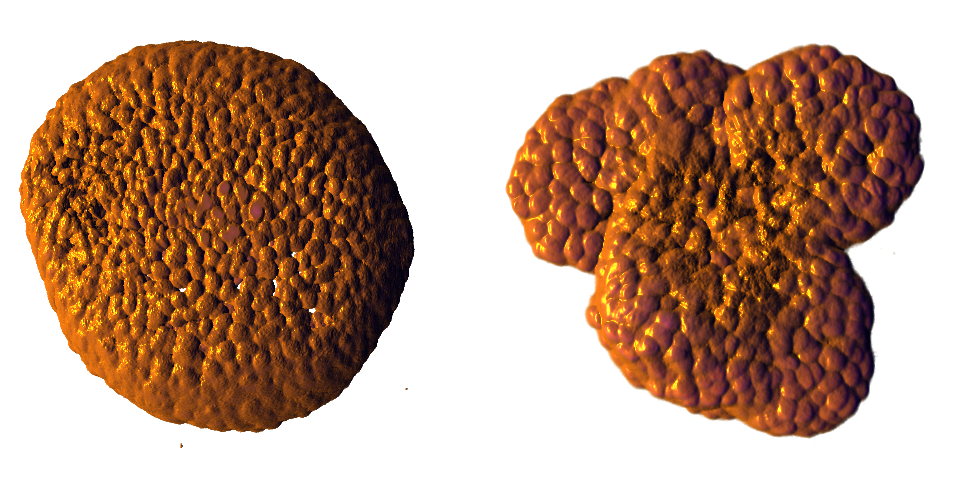
\includegraphics[width=\textwidth]{img/3Dviz.png}
            \end{center}
        \end{column}
    \end{columns}
\end{frame}

% Slide 3: The Problem
\begin{frame}{The Challenge: Automated Phenotype Classification}
    \begin{columns}
        \begin{column}{0.48\textwidth}
            \begin{block}{\textcolor{cysticGreen}{\faCheck} Cystic (Healthy)}
                \begin{itemize}
                    \item Spherical, central cavity
                    \item Organized structure
                    \item \textbf{Uniform} cell distribution
                \end{itemize}
            \end{block}
            \vspace{0.3em}
            \begin{block}{\textcolor{cauliflowerOrange}{\faExclamationTriangle} Cauliflower (Perturbed)}
                \begin{itemize}
                    \item Irregular, multiple buds
                    \item Disorganized structure
                    \item \textbf{Clustered} cell distribution
                \end{itemize}
            \end{block}
        \end{column}
        \begin{column}{0.52\textwidth}
            \begin{center}
                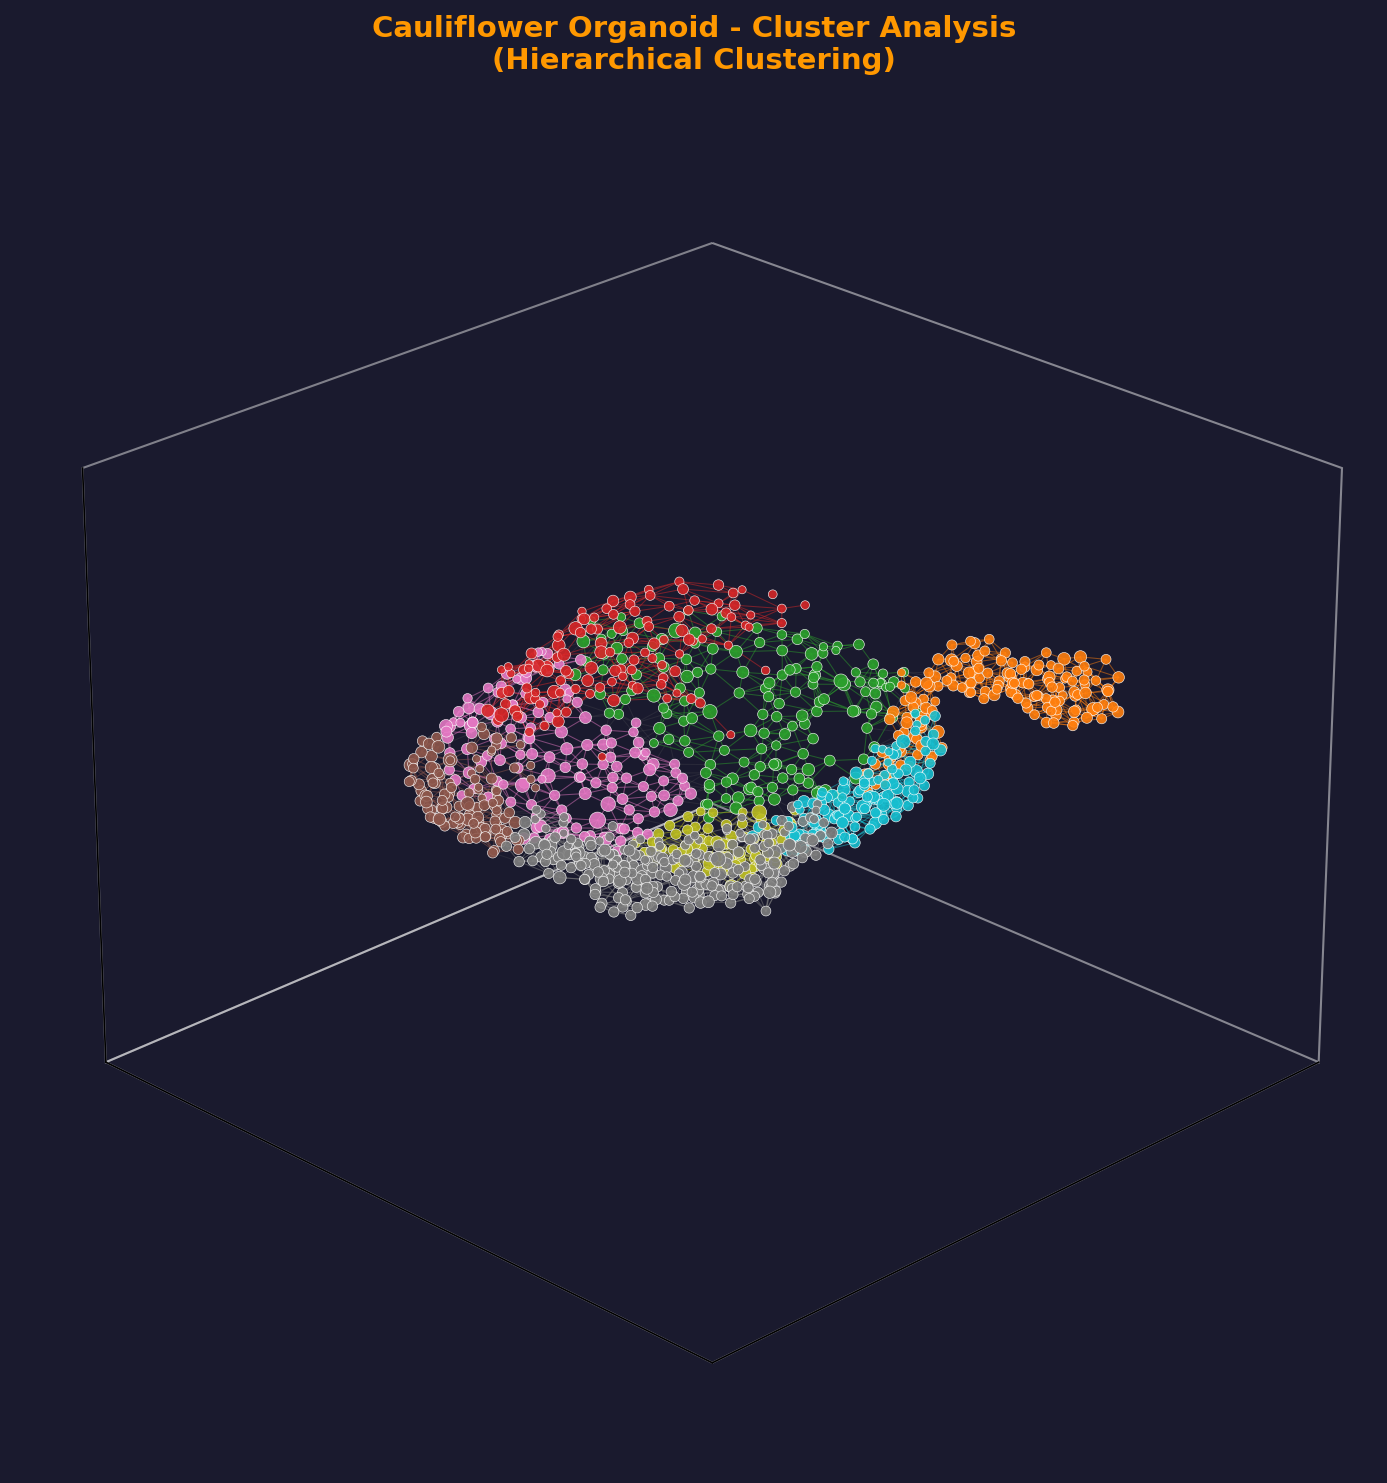
\includegraphics[width=\textwidth]{animations/real_organoid_clusters1.png}\\
                {\footnotesize Cell distribution differs between phenotypes}
            \end{center}
        \end{column}
    \end{columns}
    
    \vspace{0.5em}
    \begin{alertblock}{Goal}
        Automatically classify organoid phenotypes from 3D microscopy images
    \end{alertblock}
\end{frame}

% Slide 4: The Initial Situation
\begin{frame}{Starting Point: No Annotated Data}
    \begin{columns}
        \begin{column}{0.5\textwidth}
            \textbf{At the beginning of this thesis:}
            \begin{itemize}
                \item \textcolor{red}{\faTimes\ No labeled organoid dataset}
                \item \textcolor{red}{\faTimes\ No public benchmarks}
                \item \textcolor{red}{\faTimes\ Expert annotation = expensive}
            \end{itemize}
    
    \vspace{1em}
            \textbf{Key question:}\\
            \textit{How to develop and validate methods\\without real data?}
        \end{column}
        \begin{column}{0.5\textwidth}
    \begin{center}
                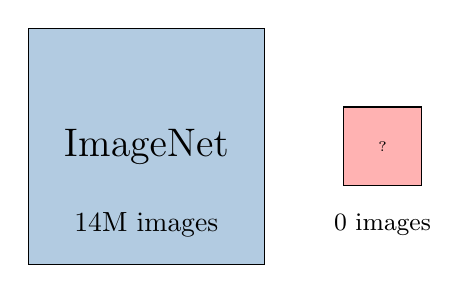
\begin{tikzpicture}
                    \draw[fill=inriaBlue!30] (0,0) rectangle (3,3);
                    \node at (1.5,1.5) {\Large ImageNet};
                    \node at (1.5,0.5) {14M images};
                    
                    \draw[fill=red!30] (4,1) rectangle (5,2);
                    \node at (4.5,1.5) {\tiny ?};
                    \node at (4.5,0.5) {\small 0 images};
                \end{tikzpicture}
    \end{center}
            
            \vspace{0.5em}
            \begin{block}{Our Approach}
                \textbf{Synthetic data} + \textbf{Graph modeling}\\to bootstrap the research
            \end{block}
        \end{column}
    \end{columns}
\end{frame}

% Slide 5: Three Challenges
\begin{frame}{Three Key Challenges}
    \begin{columns}
        \begin{column}{0.33\textwidth}
            \begin{center}
                \textbf{\faUserClock\ Challenge 1}\\[0.3em]
                \textcolor{inriaRed}{Manual Analysis}
            \end{center}
            \begin{itemize}
                \item 30 min/organoid
                \item Subjective
                \item Not reproducible
            \end{itemize}
        \end{column}
        \begin{column}{0.33\textwidth}
            \begin{center}
                \textbf{\faDatabase\ Challenge 2}\\[0.3em]
                \textcolor{inriaRed}{Data Scarcity}
            \end{center}
            \begin{itemize}
                \item No public datasets
                \item Expensive annotation
                \item Domain-specific
            \end{itemize}
        \end{column}
        \begin{column}{0.33\textwidth}
            \begin{center}
                \textbf{\faCube\ Challenge 3}\\[0.3em]
                \textcolor{inriaRed}{3D Geometry}
            \end{center}
            \begin{itemize}
                \item No preferred orientation
                \item 2 GB per organoid
                \item Rotation invariance
            \end{itemize}
        \end{column}
    \end{columns}
    
    \vspace{1em}
    \begin{alertblock}{Need}
        Automated, data-efficient, geometrically robust methods
    \end{alertblock}
\end{frame}

% Slide 6: Research Questions
\begin{frame}{Research Questions}
    \begin{enumerate}
        \item[\textbf{Q1}] \textbf{Can we model organoids as geometric graphs?}
            \begin{itemize}
            \item Capture biological information while compressing data
            \end{itemize}
            
        \vspace{0.8em}
        \item[\textbf{Q2}] \textbf{Do GNNs outperform classical spatial statistics?}
            \begin{itemize}
            \item Justify the deep learning approach
            \end{itemize}
            
        \vspace{0.8em}
        \item[\textbf{Q3}] \textbf{Can synthetic data enable transfer learning?}
        \begin{itemize}
            \item Compensate for lack of real annotations
        \end{itemize}
    \end{enumerate}
\end{frame}

% Slide 6: Outline
\begin{frame}{Presentation Outline}
    \begin{center}
        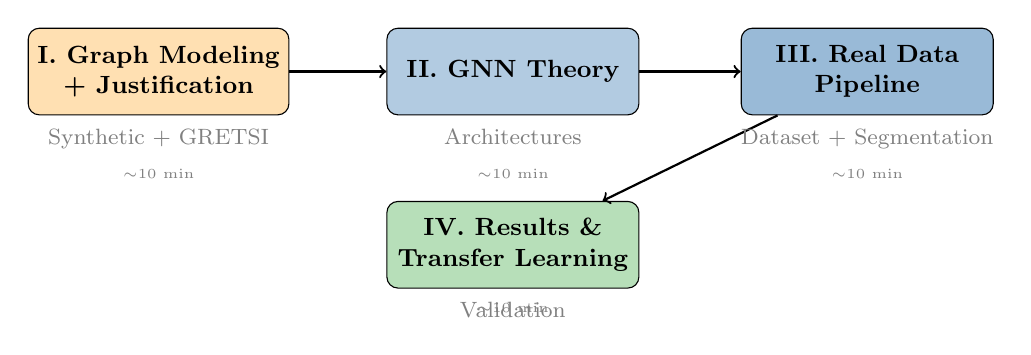
\begin{tikzpicture}[
            node distance=0.5cm,
            part/.style={rectangle, rounded corners, draw, minimum width=3.2cm, minimum height=1.1cm, align=center, font=\small\bfseries},
            time/.style={font=\tiny, text=gray}
        ]
            \node[part, fill=cauliflowerOrange!30] (p1) at (0,0) {I. Graph Modeling\\+ Justification};
            \node[part, fill=inriaBlue!30] (p2) at (4.5,0) {II. GNN Theory};
            \node[part, fill=inriaBlue!40] (p3) at (9,0) {III. Real Data\\Pipeline};
            \node[part, fill=cysticGreen!40] (p4) at (4.5,-2.2) {IV. Results \&\\Transfer Learning};
            
            \draw[->, thick] (p1) -- (p2);
            \draw[->, thick] (p2) -- (p3);
            \draw[->, thick] (p3) -- (p4);
            
            \node[time, below=0.05cm of p1] {\footnotesize Synthetic + GRETSI};
            \node[time, below=0.05cm of p2] {\footnotesize Architectures};
            \node[time, below=0.05cm of p3] {\footnotesize Dataset + Segmentation};
            \node[time, below=0.05cm of p4] {\footnotesize Validation};
            
            % Timeline
            \node[time] at (0,-1.3) {$\sim$10 min};
            \node[time] at (4.5,-1.3) {$\sim$10 min};
            \node[time] at (9,-1.3) {$\sim$10 min};
            \node[time] at (4.5,-3.0) {$\sim$10 min};
            \end{tikzpicture}
    \end{center}
    
    \vspace{0.3em}
    \begin{center}
        {\small \textbf{Narrative:} No data $\rightarrow$ Synthetic + theory $\rightarrow$ Real data arrives $\rightarrow$ Transfer learning}
    \end{center}
\end{frame}

% =============================================================================
% PART I: GRAPH MODELING & JUSTIFICATION
% =============================================================================
\section{Graph Modeling and Justification}

\begin{frame}
    \begin{center}
        {\Huge \textbf{Part I}}\\[1em]
        {\LARGE Graph Modeling \& Justification}\\[0.5em]
        {\large Why graphs? Why GNNs?}
    \end{center}
\end{frame}

% Slide 8: Why Graphs?
\begin{frame}{Why Model Organoids as Graphs?}
    \begin{columns}
        \begin{column}{0.55\textwidth}
            \textbf{Key Biological Insight:}\\
            Cell \textbf{spatial organization} differs between phenotypes
            
            \vspace{0.5em}
            \textbf{Graph Abstraction:}
            \begin{itemize}
                \item Each \textbf{cell} $\rightarrow$ \textbf{node}
                \item Spatial proximity $\rightarrow$ \textbf{edges}
                \item Node features: position $(x,y,z)$, volume
            \end{itemize}
            
            \vspace{0.5em}
            \textbf{Advantages:}
            \begin{itemize}
                \item \textbf{1000× compression} (GB $\rightarrow$ MB)
                \item Captures relational structure
                \item Natural for point cloud data
            \end{itemize}
        \end{column}
        \begin{column}{0.45\textwidth}
            \begin{center}
                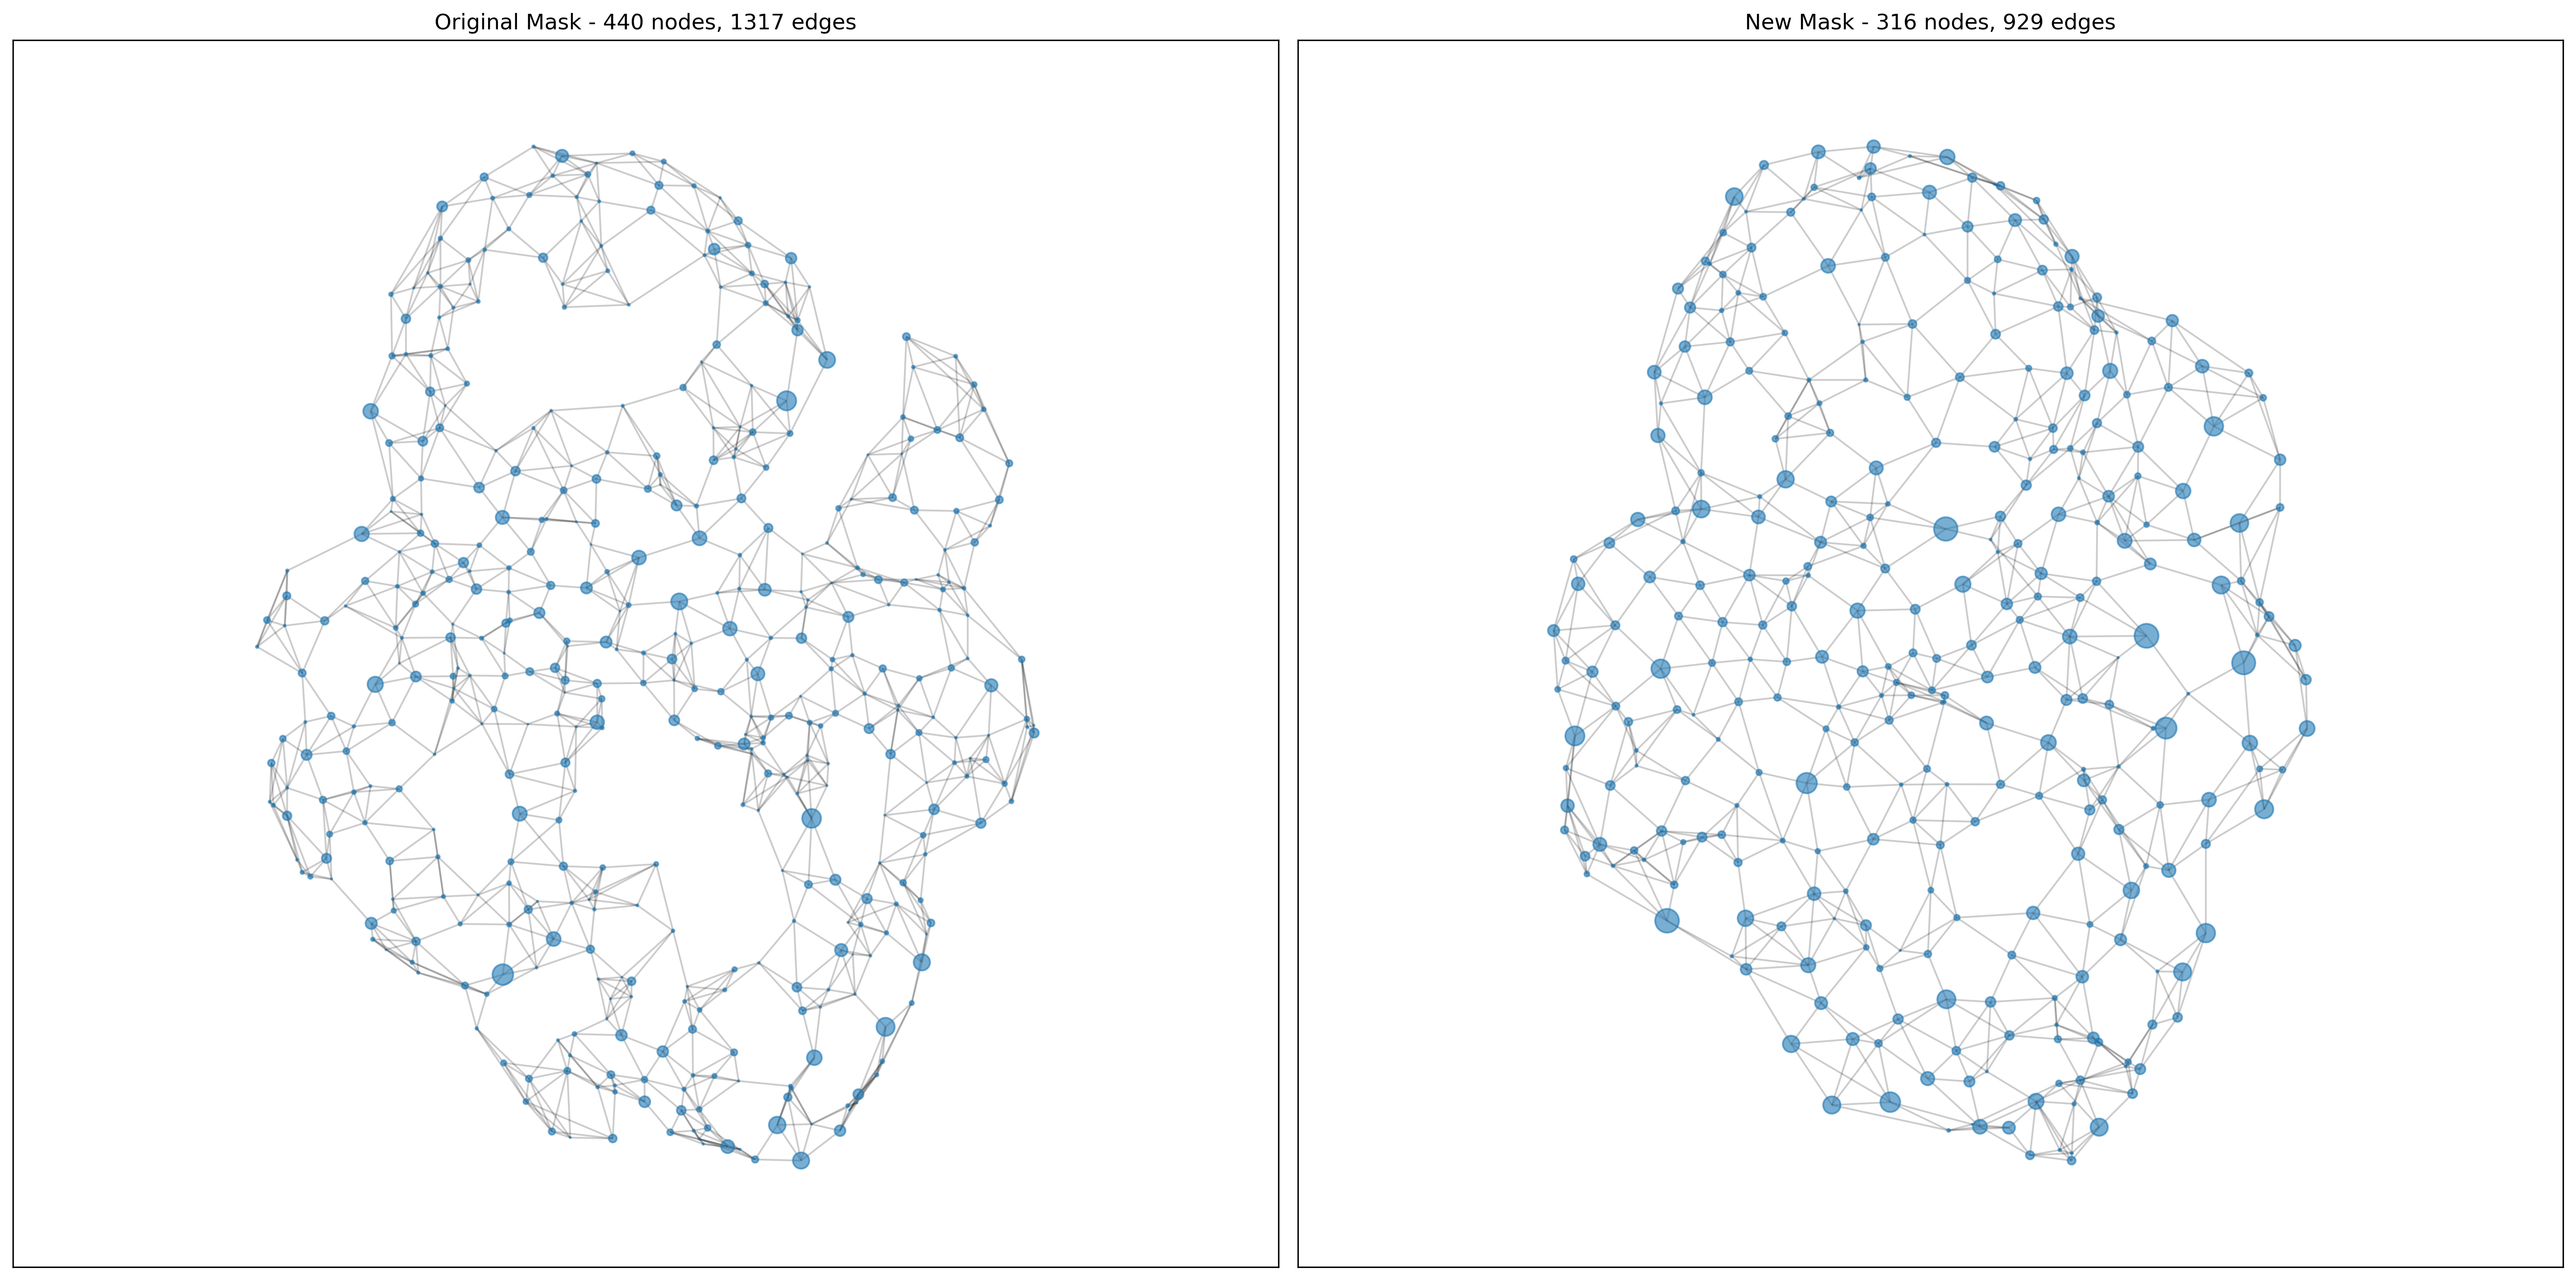
\includegraphics[width=\textwidth]{img/graph_comparison.png}
            \end{center}
        \end{column}
    \end{columns}
\end{frame}

% Slide 9: Synthetic Generation - Motivation
\begin{frame}{Synthetic Organoid Generation: Motivation}
    \begin{columns}
        \begin{column}{0.5\textwidth}
            \textbf{Problem:} No real data at thesis start
            
            \vspace{0.5em}
            \textbf{Key Biological Insight:}\\
            Cell distribution differs between phenotypes
            \begin{itemize}
                \item Cystic $\rightarrow$ \textbf{uniform} distribution
                \item Cauliflower $\rightarrow$ \textbf{clustered} distribution
            \end{itemize}
            
            \vspace{0.5em}
            \textbf{Solution:} Spatial point processes
            \begin{itemize}
                \item Mathematical models for point patterns
                \item Controllable parameters
                \item Perfect ground truth labels
            \end{itemize}
        \end{column}
        \begin{column}{0.5\textwidth}
            \begin{center}
                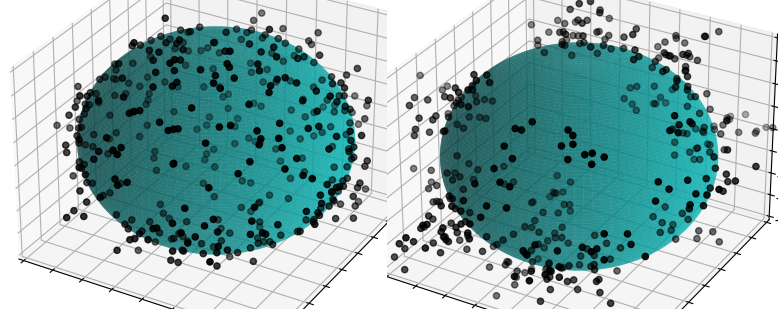
\includegraphics[width=\textwidth]{img/synthetic.png}\\
                {\footnotesize Uniform vs clustered distributions}
            \end{center}
        \end{column}
    \end{columns}
\end{frame}

% Slide 10: Point Processes Detail
\begin{frame}{Point Processes: Mathematical Foundation}
    \begin{columns}
        \begin{column}{0.5\textwidth}
            \begin{block}{\textcolor{cysticGreen}{Poisson Process} (Cystic)}
                \textbf{Intensity:} $\lambda$ (points per unit volume)
                \begin{equation*}
                    P(N(B) = k) = \frac{(\lambda|B|)^k e^{-\lambda|B|}}{k!}
                \end{equation*}
                {\small Complete spatial randomness}
            \end{block}
            
            \vspace{0.3em}
            \begin{block}{\textcolor{cauliflowerOrange}{Matérn Cluster} (Cauliflower)}
                \textbf{Parameters:}
                \begin{itemize}
                    \item $\kappa$: parent intensity
                    \item $\mu$: children per parent
                    \item $r$: cluster radius
                \end{itemize}
            \end{block}
        \end{column}
        \begin{column}{0.5\textwidth}
            \begin{center}
                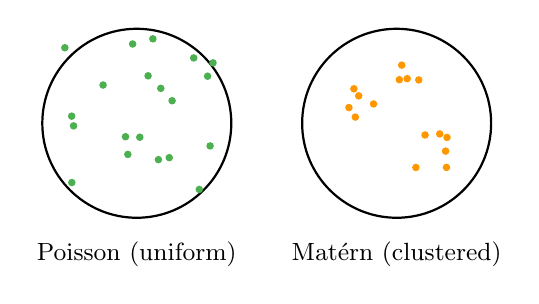
\begin{tikzpicture}[scale=0.6]
                    % Poisson
                    \draw[thick] (0,0) circle (2);
                    \foreach \i in {1,...,20} {
                        \pgfmathsetmacro{\x}{rand*1.8}
                        \pgfmathsetmacro{\y}{rand*1.8}
                        \fill[cysticGreen] (\x,\y) circle (0.08);
                    }
                    \node[below] at (0,-2.3) {\small Poisson (uniform)};
                    
                    % Matern
                    \begin{scope}[xshift=5.5cm]
                        \draw[thick] (0,0) circle (2);
                        % Cluster 1
                        \foreach \i in {1,...,5} {
                            \pgfmathsetmacro{\x}{-0.8+rand*0.4}
                            \pgfmathsetmacro{\y}{0.5+rand*0.4}
                            \fill[cauliflowerOrange] (\x,\y) circle (0.08);
                        }
                        % Cluster 2
                        \foreach \i in {1,...,6} {
                            \pgfmathsetmacro{\x}{0.7+rand*0.4}
                            \pgfmathsetmacro{\y}{-0.6+rand*0.4}
                            \fill[cauliflowerOrange] (\x,\y) circle (0.08);
                        }
                        % Cluster 3
                        \foreach \i in {1,...,4} {
                            \pgfmathsetmacro{\x}{0.2+rand*0.3}
                            \pgfmathsetmacro{\y}{1.2+rand*0.3}
                            \fill[cauliflowerOrange] (\x,\y) circle (0.08);
                        }
                        \node[below] at (0,-2.3) {\small Matérn (clustered)};
                    \end{scope}
                \end{tikzpicture}
            \end{center}
            
            \vspace{0.3em}
            {\footnotesize \faPlayCircle\ \texttt{point\_processes.gif}}
        \end{column}
    \end{columns}
\end{frame}

% Slide 11: Synthetic Dataset Statistics
\begin{frame}{Synthetic Dataset: Statistics}
    \begin{columns}
        \begin{column}{0.5\textwidth}
            \textbf{Generation Parameters:}
            \begin{itemize}
                \item Cell count: 100--500 per organoid
                \item Sphere radius: normalized to 1
                \item Volume features: log-normal distribution
            \end{itemize}
            
            \vspace{0.5em}
            \textbf{Dataset Splits:}
            \begin{table}
                \footnotesize
                \begin{tabular}{lc}
                    \toprule
                    \textbf{Split} & \textbf{Count} \\
                    \midrule
                    Training & 70,000 \\
                    Validation & 15,000 \\
                    Test & 15,000 \\
                    \midrule
                    \textbf{Total} & \textbf{100,000} \\
                    \bottomrule
                \end{tabular}
            \end{table}
        \end{column}
        \begin{column}{0.5\textwidth}
            \begin{center}
                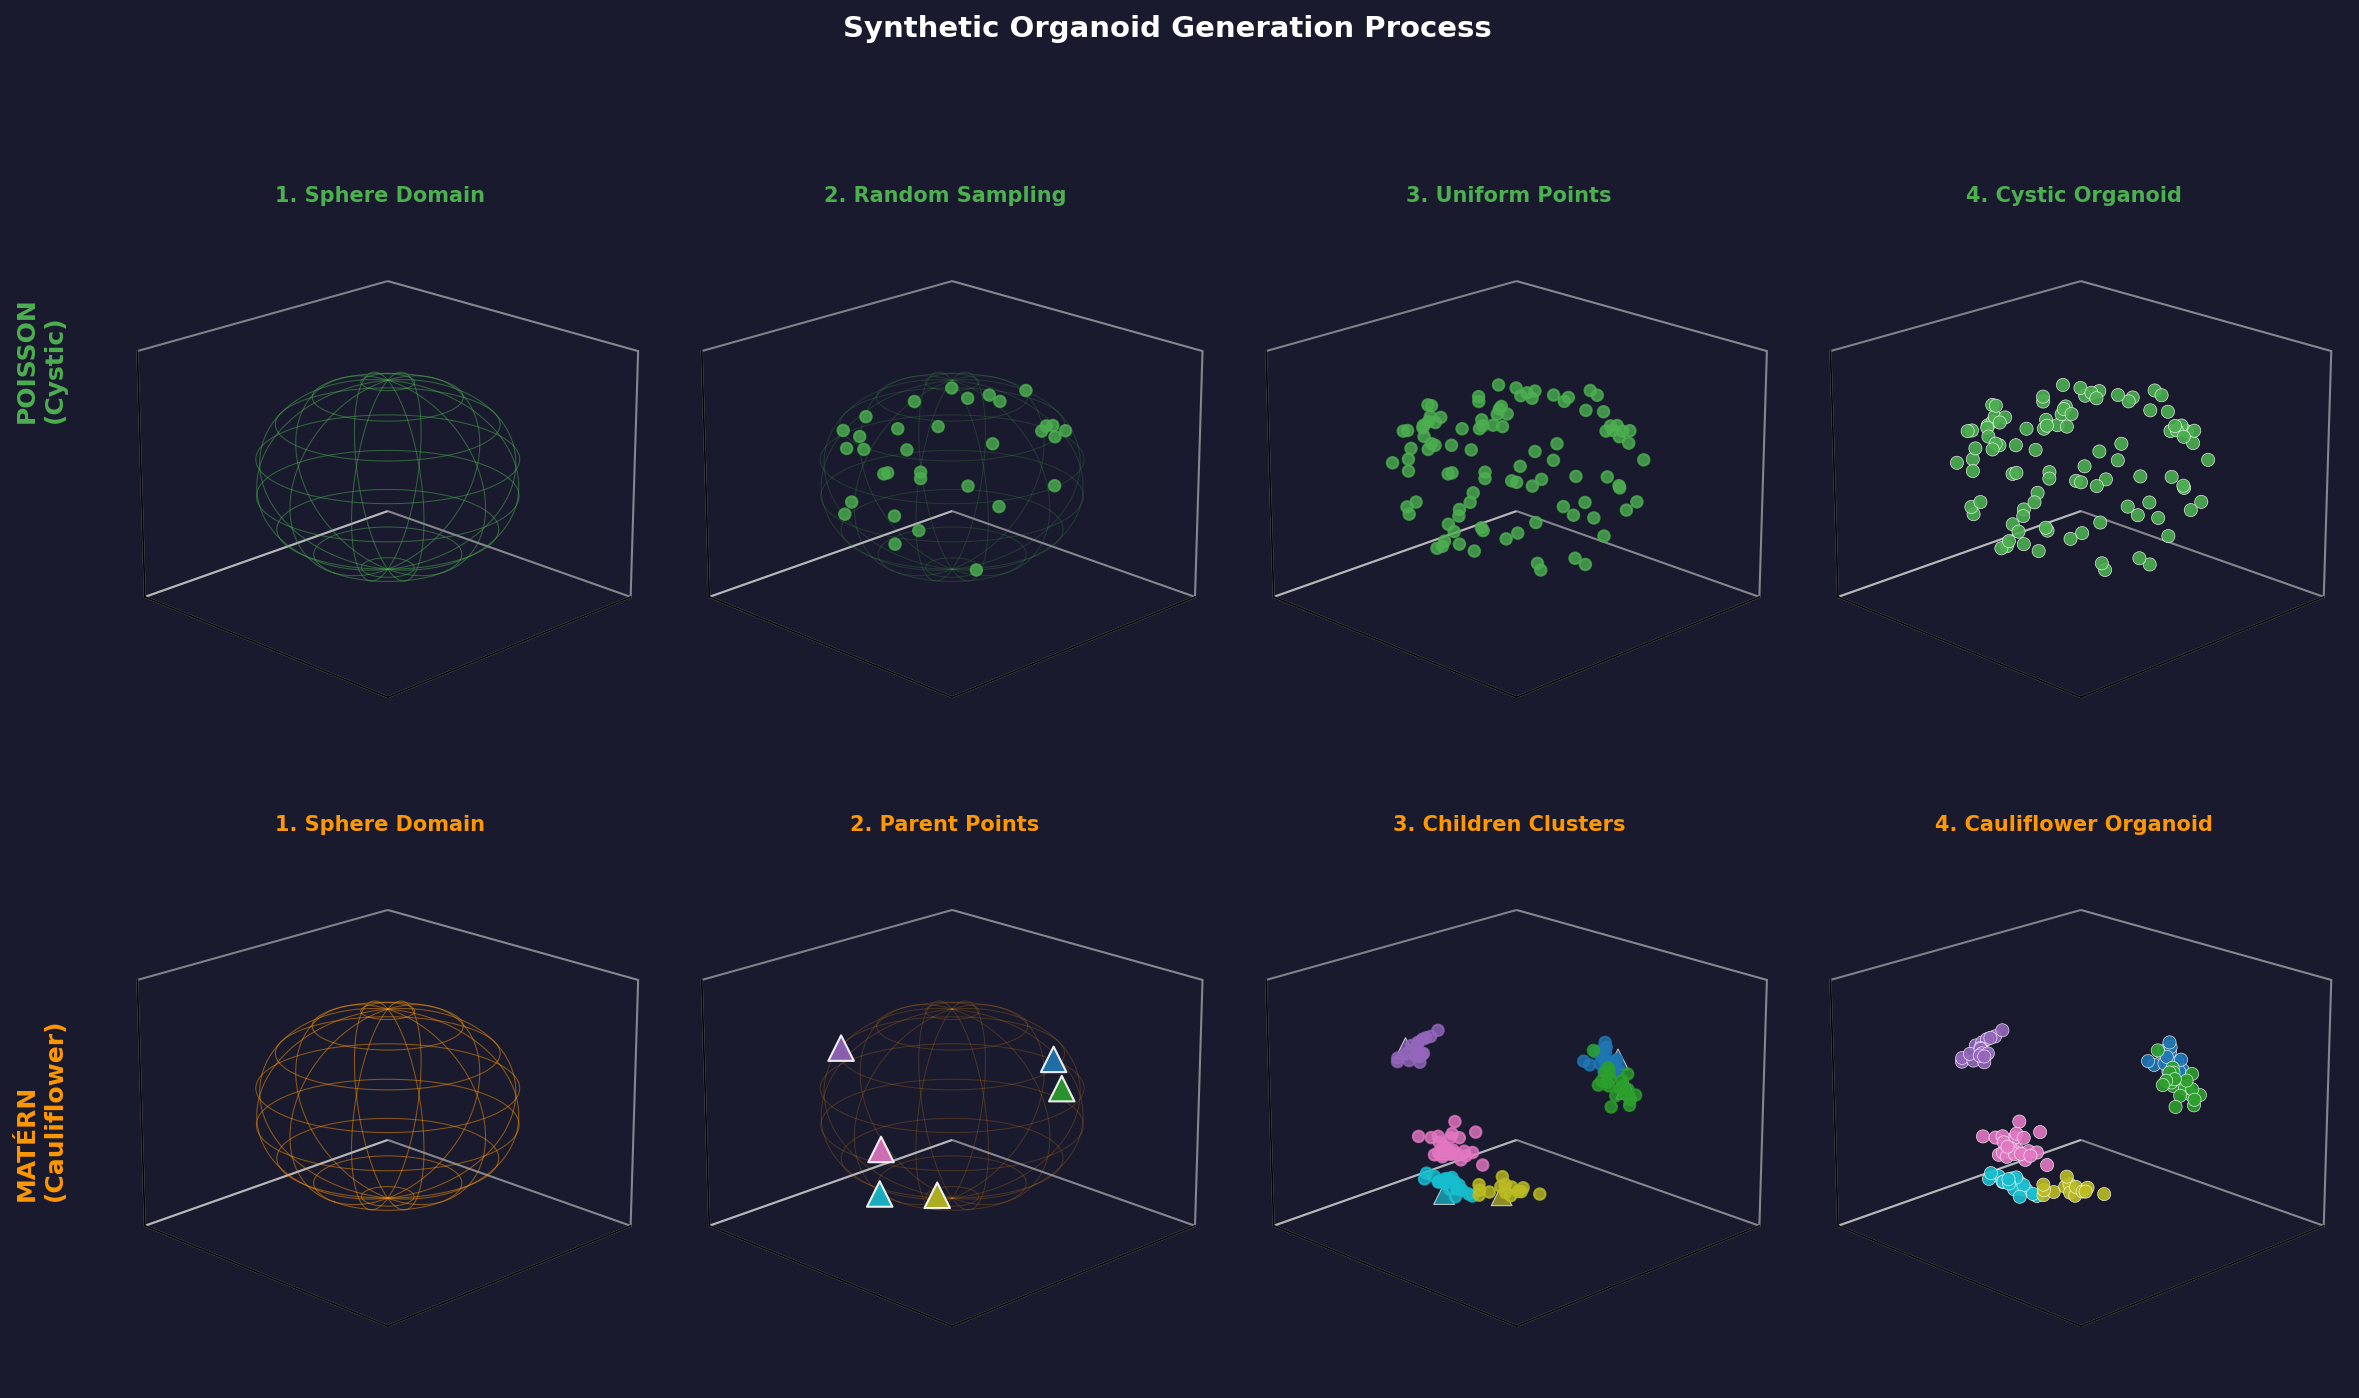
\includegraphics[width=\textwidth]{animations/synthetic_generation_steps.png}\\
                {\footnotesize Generation pipeline steps}
            \end{center}
            
            \vspace{0.3em}
            \textbf{Advantages:}
            \begin{itemize}
                \item Perfect ground truth
                \item Unlimited supply
                \item Controllable difficulty
            \end{itemize}
        \end{column}
    \end{columns}
\end{frame}

% Slide 10: GRETSI Study Introduction
\begin{frame}{GRETSI 2025: GNNs vs Spatial Statistics}
    \textbf{Research Question:}\\
    \textit{When should we prefer GNNs over classical methods?}
    
    \vspace{0.5em}
    \begin{columns}
        \begin{column}{0.5\textwidth}
            \textbf{Classical Approach:}
            \begin{itemize}
                \item Ripley's K, F, G functions
                \item Random Forest classifier
                \item Well-established in spatial statistics
            \end{itemize}
        \end{column}
        \begin{column}{0.5\textwidth}
            \textbf{Deep Learning Approach:}
            \begin{itemize}
                \item Graph Neural Networks
                \item Learn features from data
                \item End-to-end learning
            \end{itemize}
        \end{column}
    \end{columns}
    
    \vspace{0.5em}
    \textbf{Protocol:}
    \begin{itemize}
        \item Synthetic data with controlled ground truth
        \item Test noise robustness and geometric generalization
    \end{itemize}
\end{frame}

% Slide 11: Noise Robustness
\begin{frame}{Result 1: Noise Robustness}
    \begin{columns}
        \begin{column}{0.5\textwidth}
            \begin{center}
                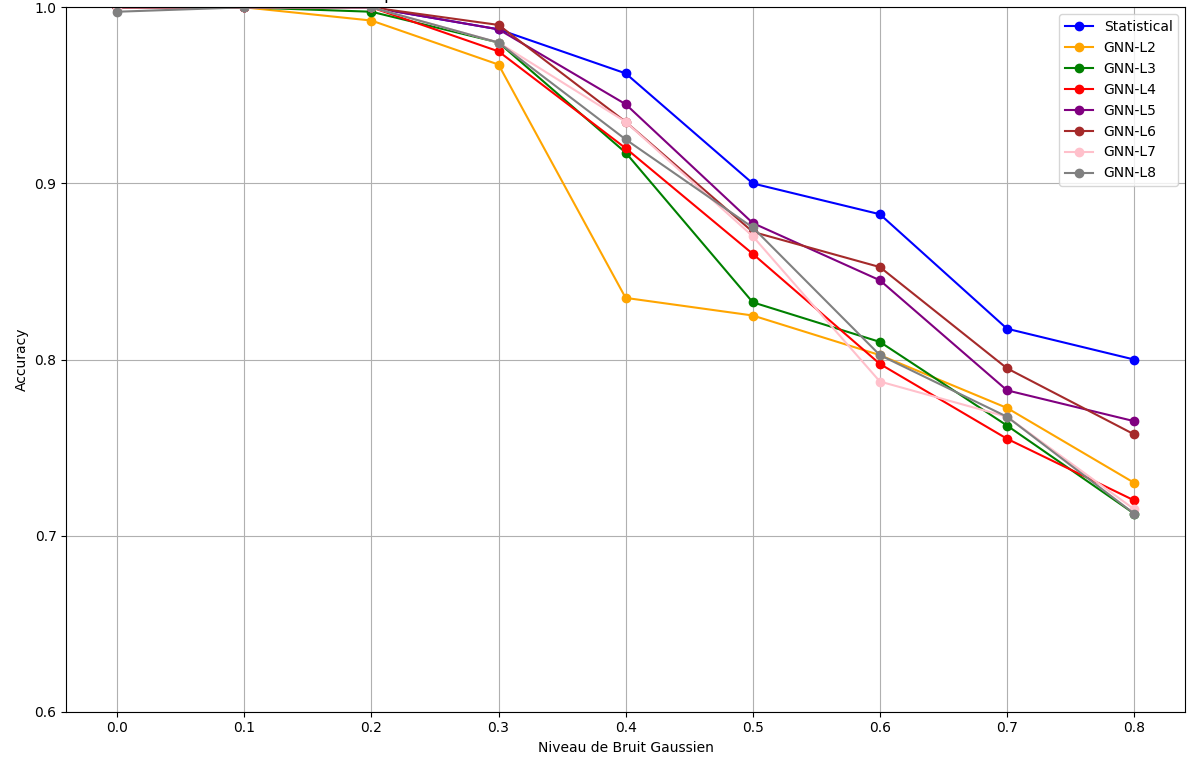
\includegraphics[width=\textwidth]{img/noise.png}
            \end{center}
        \end{column}
        \begin{column}{0.5\textwidth}
            \textbf{Observation:}\\
            Spatial statistics are \textbf{more robust to noise}
            
            \vspace{0.5em}
            \textbf{Why?}
            \begin{itemize}
                \item Ripley's functions average over many point pairs
                \item Natural smoothing effect
                \item GNNs can propagate noise through layers
            \end{itemize}
            
            \vspace{0.5em}
            \textbf{Optimal GNN depth:} 5-6 layers
            \begin{itemize}
                \item Deeper $\rightarrow$ over-smoothing
            \end{itemize}
        \end{column}
    \end{columns}
\end{frame}

% Slide 12: Geometric Generalization
\begin{frame}{Result 2: Geometric Generalization}
    \begin{columns}
        \begin{column}{0.5\textwidth}
            \begin{center}
                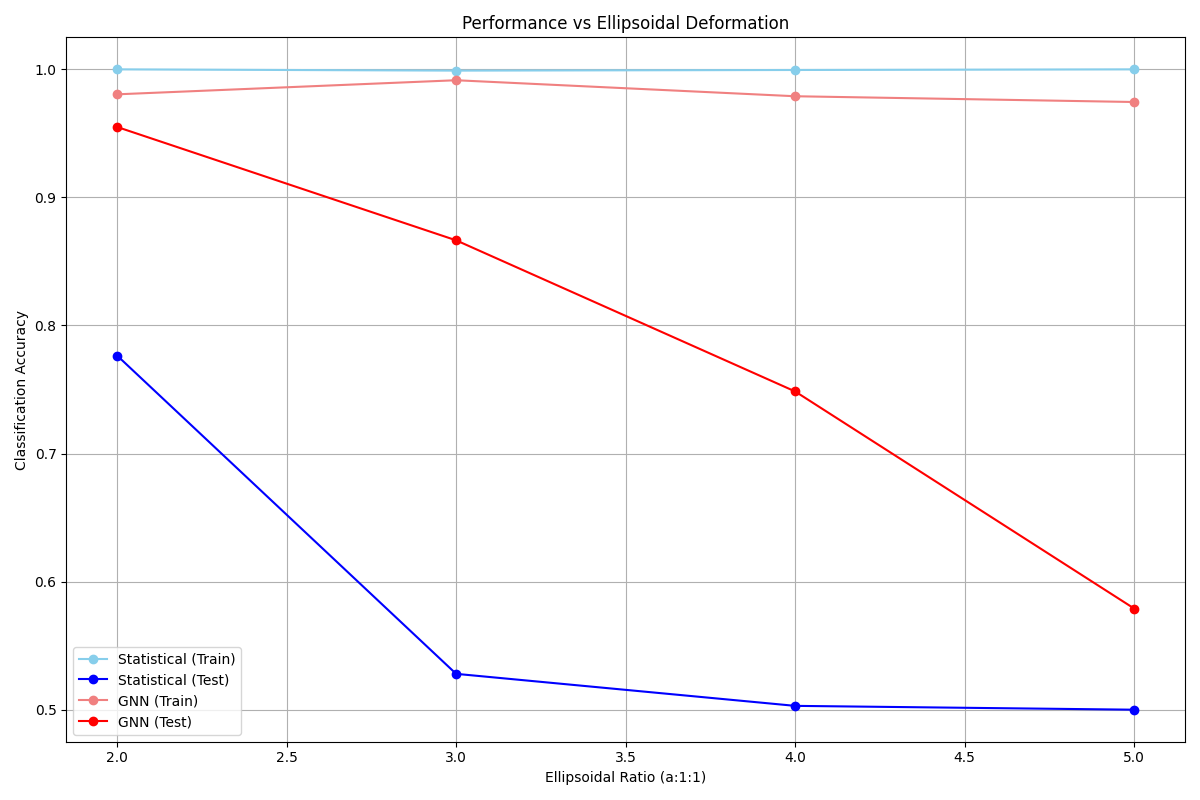
\includegraphics[width=\textwidth]{img/accuracy_vs_ratio.png}
            \end{center}
        \end{column}
        \begin{column}{0.5\textwidth}
            \textbf{Experiment:}\\
            Train on spheres, test on ellipsoids
            
            \vspace{0.5em}
            \textbf{Results:}
            \begin{itemize}
                \item Spatial stats: 100\% $\rightarrow$ 65\% (\textcolor{red}{$-$35\%})
                \item GNNs: 95\% $\rightarrow$ 82\% (\textcolor{cysticGreen}{$-$13\%})
            \end{itemize}
            
            \vspace{0.5em}
            \textbf{Why?}
            \begin{itemize}
                \item Ripley's K assumes isotropy
                \item GNNs learn \textbf{topological} patterns
            \end{itemize}
        \end{column}
    \end{columns}
    
    \vspace{0.5em}
    \begin{alertblock}{Key Finding}
        GNNs excel when morphologies vary — \textbf{exactly our situation with real organoids!}
    \end{alertblock}
\end{frame}

% Slide 13: GRETSI Conclusion
\begin{frame}{Justification: Why GNNs for Organoids}
    \begin{columns}
        \begin{column}{0.5\textwidth}
            \textbf{GNNs Excel When:}
        \begin{itemize}
                \item Morphologies vary
                \item Shapes are irregular
                \item Geometry is non-spherical
        \end{itemize}
        
            \vspace{0.5em}
            $\Rightarrow$ \textcolor{cysticGreen}{\textbf{Real organoids}}
        \end{column}
        \begin{column}{0.5\textwidth}
            \textbf{Spatial Statistics Excel When:}
        \begin{itemize}
                \item Geometry is perfectly spherical
                \item Consistent across samples
                \item Low noise environment
        \end{itemize}
        
            \vspace{0.5em}
            $\Rightarrow$ \textbf{Idealized conditions only}
        \end{column}
    \end{columns}
    
    \vspace{1em}
    \begin{block}{Foundation for Our Approach}
        For cystic vs cauliflower with variable morphologies, \textbf{GNNs are the appropriate choice}
    \end{block}
\end{frame}

% Slide 14: Part I Summary
\begin{frame}{Part I Summary: Justification}
    \begin{enumerate}
        \item \textbf{Graphs} naturally capture cellular spatial organization
        
        \vspace{0.5em}
        \item \textbf{Synthetic data} enables method development without annotations
        
        \vspace{0.5em}
        \item \textbf{GRETSI study} demonstrates:
        \begin{itemize}
            \item GNNs $>$ spatial statistics for variable morphologies
            \item Justifies our deep learning approach
        \end{itemize}
    \end{enumerate}
    
    \vspace{0.5em}
    \begin{alertblock}{Next}
        Now that we've justified GNNs, let's understand how they work
    \end{alertblock}
\end{frame}

% =============================================================================
% PART II: GNN THEORY
% =============================================================================
\section{Graph Neural Networks Theory}

\begin{frame}
    \begin{center}
        {\Huge \textbf{Part II}}\\[1em]
        {\LARGE Graph Neural Networks}\\[0.5em]
        {\large Theoretical Foundations}
    \end{center}
\end{frame}

% Slide 16: Why Not 3D CNNs
\begin{frame}{Why Not 3D CNNs?}
    \begin{columns}
        \begin{column}{0.5\textwidth}
            \textbf{Memory Constraints:}
            \begin{itemize}
                \item Single organoid: $\sim$2 GB
                \item $2048 \times 2048 \times 200$ voxels
                \item GPU memory: prohibitive
            \end{itemize}
            
            \vspace{0.5em}
            \textbf{Downsampling Issues:}
            \begin{itemize}
                \item Destroys cellular details
                \item Individual cells unresolvable
            \end{itemize}
        \end{column}
        \begin{column}{0.5\textwidth}
            \textbf{No Native Invariance:}
            \begin{itemize}
                \item Not invariant to 3D rotations
                \item Requires extensive augmentation
            \end{itemize}
            
            \vspace{0.5em}
            \textbf{Grid-Based Limitation:}
            \begin{itemize}
                \item Treats organoid as voxel grid
                \item Doesn't model cells as entities
            \end{itemize}
        \end{column}
    \end{columns}
    
    \vspace{0.5em}
    \begin{alertblock}{Conclusion}
        Graphs + GNNs overcome all these limitations
    \end{alertblock}
\end{frame}

% Slide 17: Message Passing
\begin{frame}{GNNs: Message Passing Paradigm}
    \begin{columns}
        \begin{column}{0.55\textwidth}
            \textbf{Core Idea:} Nodes exchange information
            
            \vspace{0.5em}
            \textbf{Update Rule:}
            \begin{equation*}
                h_i^{(l+1)} = \text{UPDATE}\left(h_i^{(l)}, \text{AGG}\left(\{h_j^{(l)}\}_{j \in \mathcal{N}(i)}\right)\right)
            \end{equation*}
            
            \vspace{0.5em}
            \textbf{Iterative process:}
            \begin{enumerate}
                \item Each node sends messages to neighbors
                \item Aggregate incoming messages
                \item Update node representation
            \end{enumerate}
        \end{column}
        \begin{column}{0.45\textwidth}
            \begin{center}
                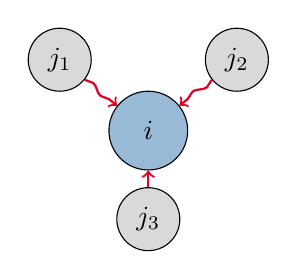
\begin{tikzpicture}[scale=0.75]
                    \node[circle, draw, fill=inriaBlue!40, minimum size=1cm] (A) at (0,0) {$i$};
                    \node[circle, draw, fill=gray!30, minimum size=0.8cm] (B) at (-1.5,1.2) {$j_1$};
                    \node[circle, draw, fill=gray!30, minimum size=0.8cm] (C) at (1.5,1.2) {$j_2$};
                    \node[circle, draw, fill=gray!30, minimum size=0.8cm] (D) at (0,-1.5) {$j_3$};
                    
                    \draw[->, thick, inriaRed, decorate, decoration={snake, amplitude=1pt}] (B) -- (A);
                    \draw[->, thick, inriaRed, decorate, decoration={snake, amplitude=1pt}] (C) -- (A);
                    \draw[->, thick, inriaRed, decorate, decoration={snake, amplitude=1pt}] (D) -- (A);
                \end{tikzpicture}\\
                {\footnotesize Messages flow to central node}\\[0.3em]
                {\tiny \faPlayCircle\ \texttt{message\_passing.gif}}
            \end{center}
        \end{column}
    \end{columns}
\end{frame}

% Slide: Global Pooling
\begin{frame}{From Node to Graph: Global Pooling}
    \textbf{Goal:} Graph-level prediction (classification), not node-level
    
    \vspace{0.5em}
    \begin{columns}
        \begin{column}{0.5\textwidth}
            \textbf{Pooling Methods:}
            \begin{itemize}
                \item \textbf{Mean:} $h_G = \frac{1}{|V|}\sum_{i \in V} h_i$
                \item \textbf{Max:} $h_G = \max_{i \in V} h_i$
                \item \textbf{Sum:} $h_G = \sum_{i \in V} h_i$
                \item \textbf{Attention:} learned weights
            \end{itemize}
            
            \vspace{0.5em}
            \textbf{Our Choice:} Mean + Max concatenation
        \end{column}
        \begin{column}{0.5\textwidth}
            \begin{center}
                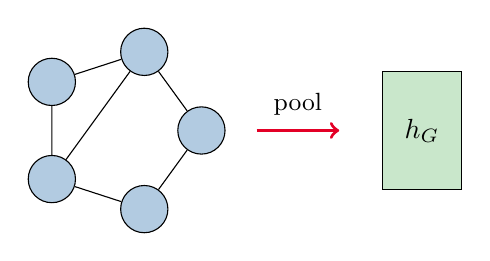
\begin{tikzpicture}[scale=0.7]
                    % Nodes
                    \foreach \i in {1,...,5} {
                        \pgfmathsetmacro{\angle}{72*\i}
                        \node[circle, draw, fill=inriaBlue!30, minimum size=0.6cm] (n\i) at (\angle:1.5) {};
                    }
                    % Edges
                    \draw (n1) -- (n2) -- (n3) -- (n4) -- (n5) -- (n1);
                    \draw (n1) -- (n3);
                    
                    % Arrow
                    \draw[->, very thick, inriaRed] (2.5,0) -- (4,0);
                    \node[above] at (3.25,0.1) {\small pool};
                    
                    % Graph embedding
                    \node[rectangle, draw, fill=cysticGreen!30, minimum width=1cm, minimum height=1.5cm] at (5.5,0) {$h_G$};
                \end{tikzpicture}
            \end{center}
        \end{column}
    \end{columns}
    
    \vspace{0.5em}
    \textbf{Classification:}
    \begin{equation*}
        \text{Nodes} \xrightarrow{\text{GNN}} \text{Embeddings} \xrightarrow{\text{Pool}} h_G \xrightarrow{\text{MLP}} \hat{y}
    \end{equation*}
\end{frame}

% Slide 18: GCN
\begin{frame}{GCN: Graph Convolutional Network (Baseline)}
    \textbf{Kipf \& Welling, 2017}
    
    \vspace{0.5em}
    \textbf{Update Rule:}
    \begin{equation*}
        h_i^{(l+1)} = \sigma\left(\sum_{j \in \mathcal{N}(i) \cup \{i\}} \frac{1}{\sqrt{d_i d_j}} W^{(l)} h_j^{(l)}\right)
    \end{equation*}
    
    \vspace{0.5em}
    \textbf{Properties:}
    \begin{itemize}
        \item Normalized mean aggregation
        \item Simple and effective baseline
        \item \textcolor{red}{\faTimes\ Treats all neighbors equally}
        \item \textcolor{red}{\faTimes\ No distance/importance weighting}
    \end{itemize}
\end{frame}

% Slide 19: GAT
\begin{frame}{GAT: Graph Attention Network}
    \textbf{Veličković et al., 2018}
    
    \vspace{0.3em}
    \textbf{Key Idea:} Learn attention coefficients to weight neighbors
    
    \begin{columns}
        \begin{column}{0.55\textwidth}
            \textbf{1. Compute attention scores:}
    \begin{equation*}
                \alpha_{ij} = \text{softmax}_j\left(\text{score}(h_i, h_j)\right)
    \end{equation*}
    
            \textbf{2. Weighted aggregation:}
    \begin{equation*}
                h_i^{\text{new}} = \sigma\left(\sum_{j \in \mathcal{N}(i)} \textcolor{inriaRed}{\alpha_{ij}} \cdot W h_j\right)
    \end{equation*}
        \end{column}
        \begin{column}{0.45\textwidth}
            \begin{center}
                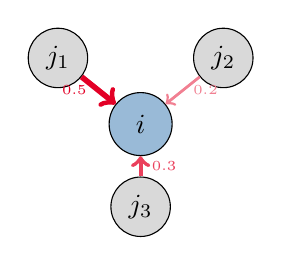
\begin{tikzpicture}[scale=0.7]
                    \node[circle, draw, fill=inriaBlue!40, minimum size=0.8cm] (A) at (0,0) {$i$};
                    \node[circle, draw, fill=gray!30, minimum size=0.6cm] (B) at (-1.5,1.2) {$j_1$};
                    \node[circle, draw, fill=gray!30, minimum size=0.6cm] (C) at (1.5,1.2) {$j_2$};
                    \node[circle, draw, fill=gray!30, minimum size=0.6cm] (D) at (0,-1.5) {$j_3$};
                    
                    \draw[->, line width=2pt, inriaRed] (B) -- (A) node[midway, left] {\tiny 0.5};
                    \draw[->, line width=1pt, inriaRed!50] (C) -- (A) node[midway, right] {\tiny 0.2};
                    \draw[->, line width=1.5pt, inriaRed!75] (D) -- (A) node[midway, right] {\tiny 0.3};
                \end{tikzpicture}\\
                {\footnotesize Learned attention weights}
            \end{center}
        \end{column}
    \end{columns}
    
    \vspace{0.3em}
    \textcolor{cysticGreen}{\faCheck} \textbf{Best performance} in our experiments
\end{frame}

% Slide 20: DeepSets
\begin{frame}{DeepSets: Set-Based Baseline}
    \textbf{Zaheer et al., 2017}
    
    \vspace{0.5em}
    \textbf{Approach:} Treat organoid as unordered set of cells (ignore edges)
    
    \begin{equation*}
        f(X) = \rho\left(\sum_{x \in X} \phi(x)\right)
    \end{equation*}
    
    \vspace{0.5em}
    \textbf{Properties:}
    \begin{itemize}
        \item Permutation invariant
        \item \textcolor{red}{\faTimes\ Ignores local spatial structure}
        \item Each cell processed independently before aggregation
    \end{itemize}
    
    \vspace{0.5em}
    \textbf{Observation:} Performs reasonably well\\
    $\Rightarrow$ Global statistics are informative, but \textbf{local structure helps}
\end{frame}

% Slide 21: Geometric Equivariance
\begin{frame}{Geometric Equivariance: Why It Matters}
    \begin{columns}
        \begin{column}{0.5\textwidth}
            \textbf{Problem:}\\
            Organoids have no preferred orientation in 3D culture
            
            \vspace{0.8em}
            \begin{block}{Invariance (for classification)}
                $f(R \cdot x) = f(x)$\\
                {\small Same prediction after rotation}
            \end{block}
            
            \vspace{0.3em}
            \begin{block}{Equivariance (for features)}
                $f(R \cdot x) = R \cdot f(x)$\\
                {\small Features rotate coherently}
            \end{block}
        \end{column}
        \begin{column}{0.5\textwidth}
            \begin{center}
                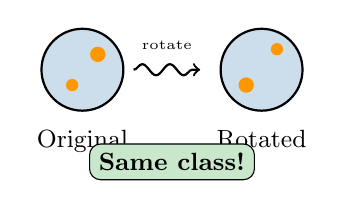
\begin{tikzpicture}[scale=0.65]
                    \draw[thick, fill=inriaBlue!20] (0,1.5) circle (0.8);
                    \fill[cauliflowerOrange] (0.3,1.8) circle (0.15);
                    \fill[cauliflowerOrange] (-0.2,1.2) circle (0.12);
                    \node[below] at (0,0.5) {\small Original};
                    
                    \draw[thick, fill=inriaBlue!20] (3.5,1.5) circle (0.8);
                    \fill[cauliflowerOrange] (3.2,1.2) circle (0.15);
                    \fill[cauliflowerOrange] (3.8,1.9) circle (0.12);
                    \node[below] at (3.5,0.5) {\small Rotated};
                    
                    \draw[->, thick, decorate, decoration={snake, amplitude=2pt}] (1,1.5) -- (2.3,1.5);
                    \node[above] at (1.65,1.7) {\tiny rotate};
                    
                    \node[draw, rounded corners, fill=cysticGreen!30, font=\small\bfseries] at (1.75,-0.3) {Same class!};
                \end{tikzpicture}\\
                {\footnotesize \faPlayCircle\ \texttt{rotation\_invariance.gif}}
            \end{center}
        \end{column}
    \end{columns}
\end{frame}

% Slide: E(3) Group
\begin{frame}{The E(3) Group: 3D Euclidean Symmetries}
    \textbf{E(3) = Euclidean group in 3 dimensions}
    
    \vspace{0.5em}
    \begin{columns}
        \begin{column}{0.33\textwidth}
            \begin{center}
                \textbf{Rotations}\\[0.3em]
                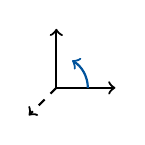
\begin{tikzpicture}[scale=0.5]
                    \draw[thick, ->] (0,0) -- (1.5,0);
                    \draw[thick, ->] (0,0) -- (0,1.5);
                    \draw[thick, dashed, ->] (0,0) -- (-0.7,-0.7);
                    \draw[thick, inriaBlue, ->] (0.8,0) arc (0:60:0.8);
                \end{tikzpicture}\\
                {\small Any 3D rotation\\around any axis}
            \end{center}
        \end{column}
        \begin{column}{0.33\textwidth}
            \begin{center}
                \textbf{Translations}\\[0.3em]
                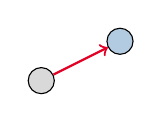
\begin{tikzpicture}[scale=0.5]
                    \node[circle, draw, fill=gray!30] (a) at (0,0) {};
                    \node[circle, draw, fill=inriaBlue!30] (b) at (2,1) {};
                    \draw[->, thick, inriaRed] (a) -- (b);
                \end{tikzpicture}\\
                {\small Shifting the entire\\structure in space}
            \end{center}
        \end{column}
        \begin{column}{0.33\textwidth}
            \begin{center}
                \textbf{Reflections}\\[0.3em]
                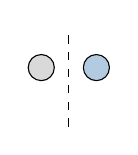
\begin{tikzpicture}[scale=0.5]
                    \draw[dashed] (0,-1) -- (0,1.5);
                    \node[circle, draw, fill=gray!30] at (-0.7,0.5) {};
                    \node[circle, draw, fill=inriaBlue!30] at (0.7,0.5) {};
                \end{tikzpicture}\\
                {\small Mirror\\symmetries}
            \end{center}
        \end{column}
    \end{columns}
    
    \vspace{1em}
    \begin{alertblock}{Key Insight}
        We can build architectures that \textbf{guarantee} these invariances by construction — not learned through augmentation, but \textbf{mathematically proven}.
    \end{alertblock}
\end{frame}

% Slide 22: EGNN
\begin{frame}{EGNN: Equivariant Graph Neural Network}
    \textbf{Satorras et al., 2021}
    
    \vspace{0.5em}
    \textbf{Key Principle:} Use only \textbf{invariant quantities} in messages
    
    \begin{columns}
        \begin{column}{0.55\textwidth}
            \textbf{Message} (uses distance = invariant):
    \begin{equation*}
        m_{ij} = \phi_m\left(h_i, h_j, \|x_i - x_j\|^2\right)
    \end{equation*}
    
    \textbf{Coordinate update} (equivariant):
    \begin{equation*}
                x_i^{new} = x_i + \sum_{j} (x_i - x_j) \cdot \phi_x(m_{ij})
    \end{equation*}
        \end{column}
        \begin{column}{0.45\textwidth}
            \textbf{Advantages:}
            \begin{itemize}
                \item \textcolor{cysticGreen}{\faCheck} No augmentation needed
                \item \textcolor{cysticGreen}{\faCheck} Guaranteed robustness
                \item \textcolor{cysticGreen}{\faCheck} Better with less data
            \end{itemize}
    
            \vspace{0.3em}
            \textbf{Trade-off:}\\
            Slightly lower raw accuracy
        \end{column}
    \end{columns}
\end{frame}

% Slide 23: Architecture Comparison
\begin{frame}{Architecture Comparison Summary}
    \begin{table}
        \centering
        \begin{tabular}{lccc}
            \toprule
            \textbf{Architecture} & \textbf{Aggregation} & \textbf{E(3)-Equiv.} & \textbf{Strength} \\
            \midrule
            GCN & Mean & \textcolor{red}{\faTimes} & Simple baseline \\
            \textbf{GAT} & Attention & \textcolor{red}{\faTimes} & \textbf{Best accuracy} \\
            DeepSets & Global sum & \textcolor{red}{\faTimes} & No local structure \\
            \textbf{EGNN} & Distance-based & \textcolor{cysticGreen}{\faCheck} & \textbf{Guaranteed robustness} \\
            \bottomrule
        \end{tabular}
    \end{table}
    
    \vspace{1em}
    \textbf{Key Trade-off:}\\
    \begin{itemize}
        \item GAT $\rightarrow$ Best raw performance
        \item EGNN $\rightarrow$ Guaranteed geometric invariance
    \end{itemize}
\end{frame}

% Slide 24: Part II Summary
\begin{frame}{Part II Summary: GNN Theory}
    \begin{enumerate}
        \item \textbf{Message passing} enables learning on graphs
        
        \vspace{0.5em}
        \item \textbf{GAT} with attention achieves best accuracy
        
        \vspace{0.5em}
        \item \textbf{EGNN} provides guaranteed E(3)-equivariance
        
        \vspace{0.5em}
        \item \textbf{All architectures} outperform spatial statistics on variable morphologies
    \end{enumerate}
    
    \vspace{0.5em}
    \begin{alertblock}{Next}
        Real data finally arrives — how to build the processing pipeline?
    \end{alertblock}
\end{frame}

% =============================================================================
% PART III: REAL DATA PIPELINE
% =============================================================================
\section{Real Data Pipeline}

\begin{frame}
    \begin{center}
        {\Huge \textbf{Part III}}\\[1em]
        {\LARGE From Real Images to Graphs}\\[0.5em]
        {\large Processing Pipeline}
    \end{center}
\end{frame}

% Slide 26: Dataset
\begin{frame}{The Real Dataset Arrives}
    \begin{columns}
        \begin{column}{0.5\textwidth}
            \textbf{ANR Morpheus Project}
            \begin{itemize}
                \item 22 months of data collection
                \item May 2023 -- February 2025
                \item IPMC Nice + Paris Cité
            \end{itemize}
            
            \vspace{0.5em}
            \textbf{Dataset Statistics:}
            \begin{itemize}
                \item 1,311 imaged samples
                \item 2,272 extracted organoids
                \item \textbf{500 well-differentiated} selected
                \item $\sim$250 per class
            \end{itemize}
        \end{column}
        \begin{column}{0.5\textwidth}
            \begin{center}
                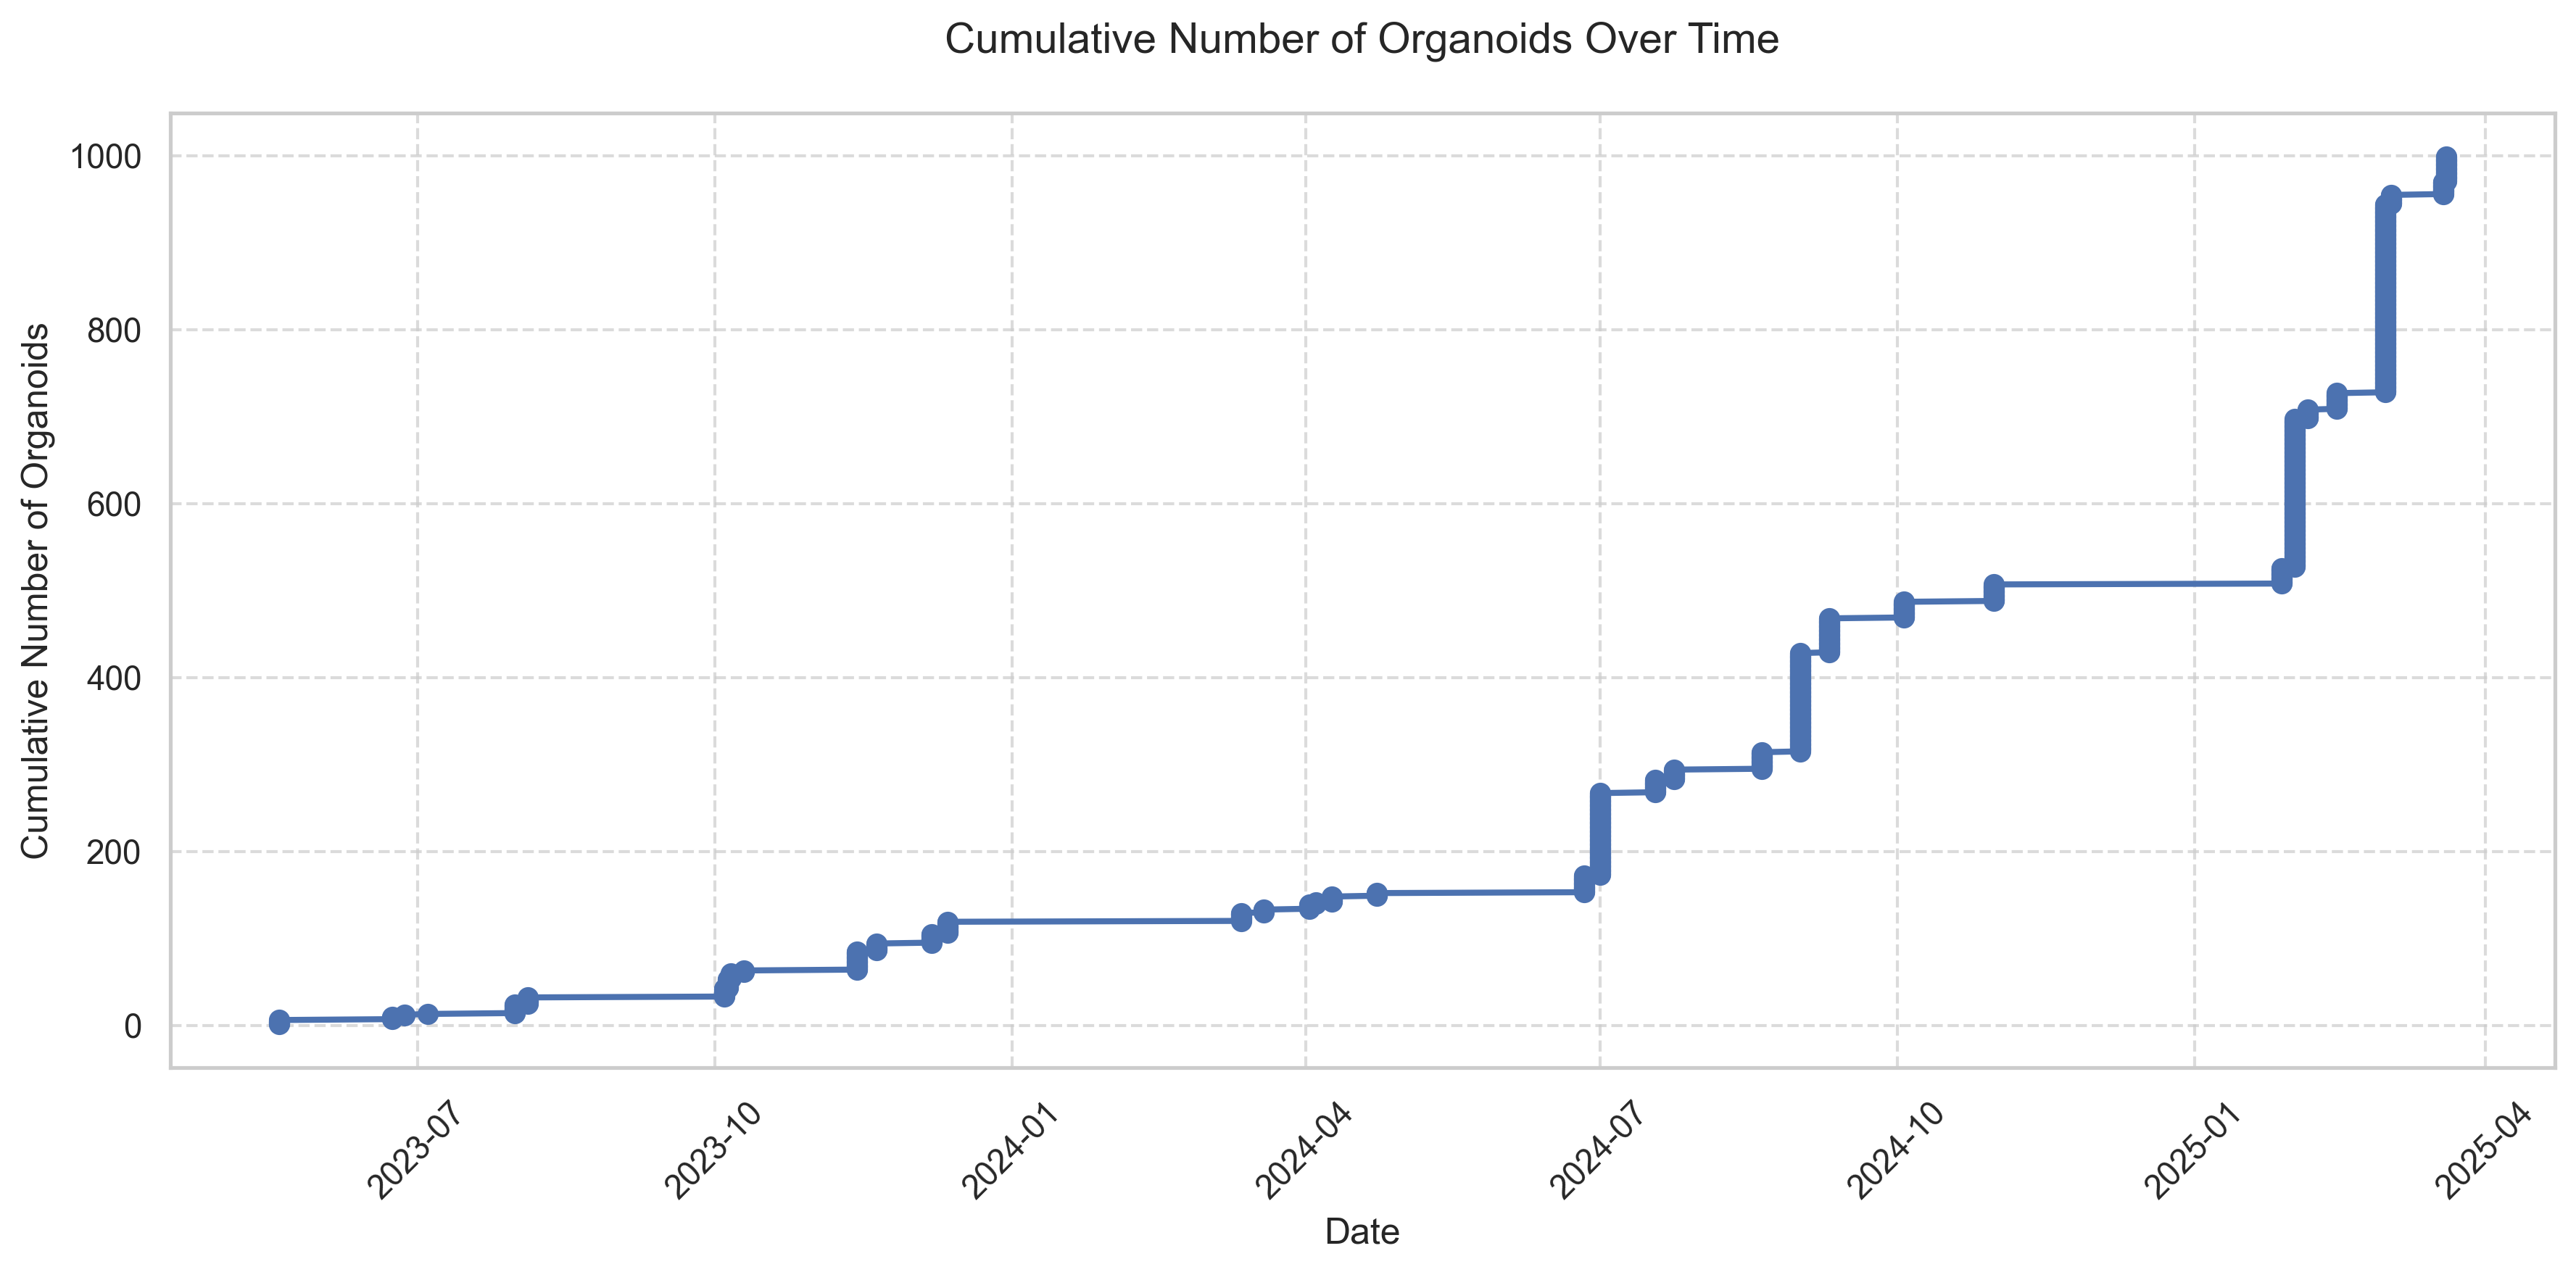
\includegraphics[width=\textwidth]{img/cumulative_organoids.png}\\
                {\footnotesize Data accumulated over 22 months}
            \end{center}
        \end{column}
    \end{columns}
    
    \vspace{0.3em}
    \begin{block}{Challenge}
        How to transform 2 GB 3D images into graphs for GNN processing?
    \end{block}
\end{frame}

% Slide 27: Pipeline Overview
\begin{frame}{End-to-End Processing Pipeline}
    \begin{center}
        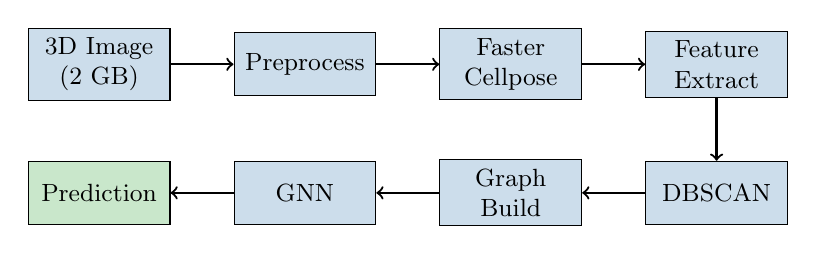
\begin{tikzpicture}[
            node distance=0.8cm,
            block/.style={rectangle, draw, fill=inriaBlue!20, minimum width=1.8cm, minimum height=0.8cm, align=center, font=\small},
            arrow/.style={->, thick}
        ]
            \node[block] (img) {3D Image\\(2 GB)};
            \node[block, right=of img] (prep) {Preprocess};
            \node[block, right=of prep] (seg) {Faster\\Cellpose};
            \node[block, right=of seg] (feat) {Feature\\Extract};
            \node[block, below=of feat] (clust) {DBSCAN};
            \node[block, left=of clust] (graph) {Graph\\Build};
            \node[block, left=of graph] (gnn) {GNN};
            \node[block, left=of gnn, fill=cysticGreen!30] (pred) {Prediction};
            
            \draw[arrow] (img) -- (prep);
            \draw[arrow] (prep) -- (seg);
            \draw[arrow] (seg) -- (feat);
            \draw[arrow] (feat) -- (clust);
            \draw[arrow] (clust) -- (graph);
            \draw[arrow] (graph) -- (gnn);
            \draw[arrow] (gnn) -- (pred);
        \end{tikzpicture}
    \end{center}
    
    \vspace{0.5em}
    \begin{columns}
        \begin{column}{0.5\textwidth}
            \textbf{Processing time:} $\sim$20 min/organoid\\
            {\footnotesize (dominated by segmentation)}
        \end{column}
        \begin{column}{0.5\textwidth}
            \textbf{Compression:} 2 GB $\rightarrow$ 10 MB\\
            {\footnotesize (\textbf{1000× reduction})}
        \end{column}
    \end{columns}
\end{frame}

% Slide 28: Segmentation
\begin{frame}{Faster Cellpose: Segmentation Bottleneck}
    \textbf{Problem:} Cellpose is slow
    \begin{itemize}
        \item 30 sec/slice × 200 slices × 1000 organoids = \textbf{2,500 hours}
    \end{itemize}
    
    \vspace{0.5em}
    \textbf{Our Solution: Faster Cellpose}
    \begin{enumerate}
        \item \textbf{Knowledge Distillation:} Smaller student network ($-$50\% params)
        \item \textbf{Weight Pruning:} Remove 30\% low-magnitude weights
        \item \textbf{Mixed Precision:} FP16 inference
    \end{enumerate}
    
    \vspace{0.5em}
    \begin{table}
        \centering
        \footnotesize
        \begin{tabular}{lccc}
            \toprule
            \textbf{Method} & \textbf{F1} & \textbf{Time/Slice} & \textbf{Speed-up} \\
            \midrule
            Geometric (ellipses) & 0.88 & 3 sec & 10× \\
            \textbf{Faster Cellpose} & \textbf{0.95} & \textbf{6 sec} & \textbf{5×} \\
            Original Cellpose & 0.98 & 30 sec & 1× \\
            \bottomrule
        \end{tabular}
    \end{table}
\end{frame}

% Slide 29: Graph Construction
\begin{frame}{Graph Construction from Segmented Cells}
    \begin{columns}
        \begin{column}{0.5\textwidth}
            \textbf{Node Features (4D):}
            \begin{itemize}
                \item 3D centroid: $(x, y, z)$
                \item Cell volume
                \item Normalized (centered, scaled)
            \end{itemize}
            
            \vspace{0.5em}
            \textbf{Edge Construction:}
            \begin{itemize}
                \item K-nearest neighbors ($K=10$)
                \item Euclidean distance
                \item Symmetrized + radial cutoff
            \end{itemize}
            
            \vspace{0.3em}
            {\footnotesize \faPlayCircle\ \texttt{graph\_construction.gif}}
        \end{column}
        \begin{column}{0.5\textwidth}
            \begin{center}
                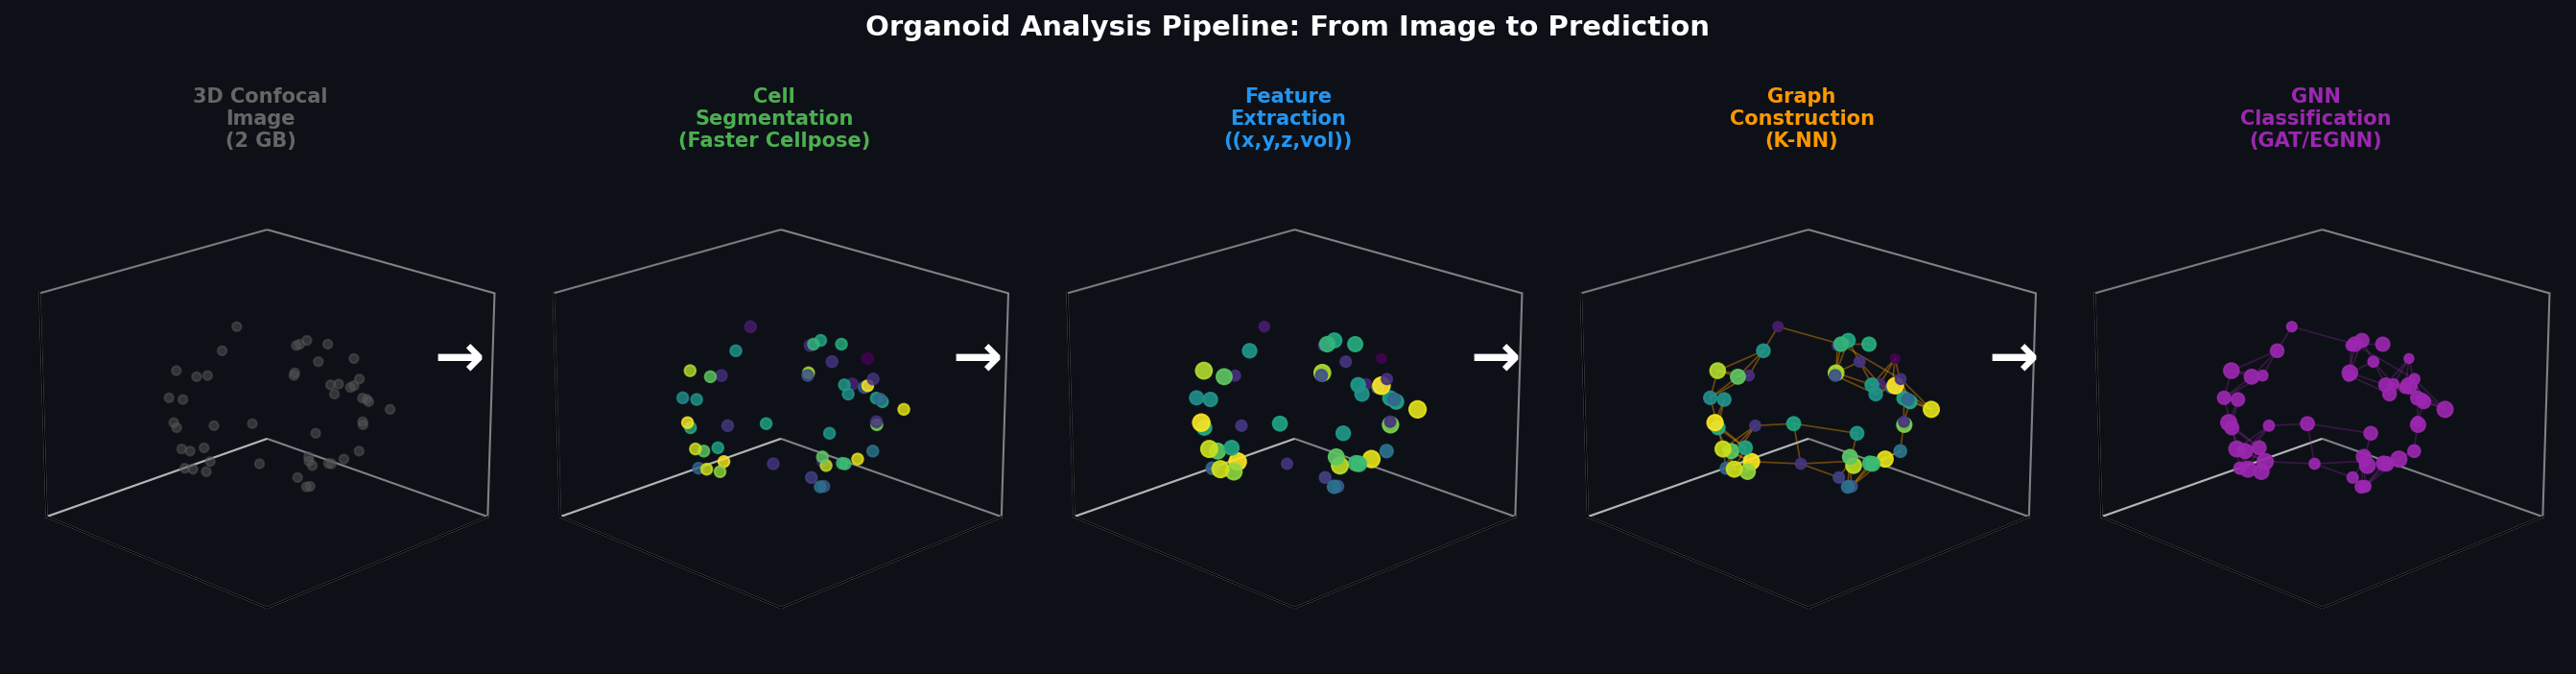
\includegraphics[width=\textwidth]{animations/graph_construction_pipeline1.png}\\
                {\footnotesize From segmentation to graph}
            \end{center}
        \end{column}
    \end{columns}
\end{frame}

% Slide 30: Part III Summary
\begin{frame}{Part III Summary: Pipeline}
    \begin{enumerate}
        \item \textbf{Real dataset:} 500 well-differentiated organoids (22 months)
    
    \vspace{0.5em}
        \item \textbf{Faster Cellpose:} 5× speedup while maintaining F1 = 0.95
    
    \vspace{0.5em}
        \item \textbf{Graph construction:} 1000× compression preserving structure
            
            \vspace{0.5em}
        \item \textbf{Complete pipeline:} 3D image $\rightarrow$ graph $\rightarrow$ prediction
    \end{enumerate}
            
            \vspace{0.5em}
    \begin{alertblock}{Next}
        Transfer learning: can synthetic pre-training help with real data?
    \end{alertblock}
\end{frame}

% =============================================================================
% PART IV: RESULTS & TRANSFER LEARNING
% =============================================================================
\section{Results and Transfer Learning}

\begin{frame}
    \begin{center}
        {\Huge \textbf{Part IV}}\\[1em]
        {\LARGE Results \& Transfer Learning}\\[0.5em]
        {\large From Synthetic to Real}
    \end{center}
\end{frame}

% Slide 32: Transfer Learning Strategy
\begin{frame}{Transfer Learning: Synthetic $\rightarrow$ Real}
            \begin{center}
        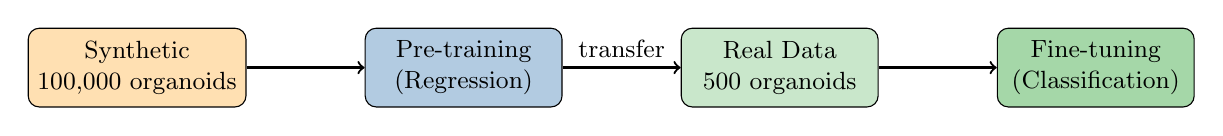
\begin{tikzpicture}[
            node distance=1cm,
            block/.style={rectangle, rounded corners, draw, minimum width=2.5cm, minimum height=1cm, align=center, font=\small},
            arrow/.style={->, thick}
        ]
            \node[block, fill=cauliflowerOrange!30] (synth) {Synthetic\\100,000 organoids};
            \node[block, fill=inriaBlue!30, right=1.5cm of synth] (pretrain) {Pre-training\\(Regression)};
            \node[block, fill=cysticGreen!30, right=1.5cm of pretrain] (real) {Real Data\\500 organoids};
            \node[block, fill=cysticGreen!50, right=1.5cm of real] (finetune) {Fine-tuning\\(Classification)};
            
            \draw[arrow] (synth) -- (pretrain);
            \draw[arrow] (pretrain) -- (real) node[midway, above] {\small transfer};
            \draw[arrow] (real) -- (finetune);
        \end{tikzpicture}
            \end{center}
            
            \vspace{0.5em}
    \begin{columns}
        \begin{column}{0.5\textwidth}
            \textbf{Phase 1: Pre-training}
            \begin{itemize}
                \item 70,000 synthetic organoids
                \item Task: Regress Matérn parent number
                \item Learn spatial organization patterns
            \end{itemize}
        \end{column}
        \begin{column}{0.5\textwidth}
            \textbf{Phase 2: Fine-tuning}
            \begin{itemize}
                \item 500 real organoids
                \item Reinitialize classification head
                \item Reduced learning rate ($10^{-4}$)
            \end{itemize}
        \end{column}
    \end{columns}
\end{frame}

% Slide 33: Synthetic Results
\begin{frame}{Performance on Synthetic Data}
    \textbf{Task:} Regression of Matérn parent number\\
    \textbf{Test set:} 15,000 synthetic organoids
    
    \vspace{0.5em}
    \begin{table}
        \centering
        \begin{tabular}{lcc}
            \toprule
            \textbf{Architecture} & \textbf{MSE} & \textbf{vs GCN} \\
            \midrule
            GCN (baseline) & 0.198 & — \\
            DeepSets & 0.145 & +27\% \\
            EGNN & 0.137 & +31\% \\
            \textbf{GAT} & \textbf{0.118} & \textbf{+40\%} \\
            \bottomrule
        \end{tabular}
    \end{table}
    
    \vspace{0.5em}
    \textbf{Key findings:}
    \begin{itemize}
        \item GAT wins: attention learns which neighbors matter
        \item EGNN: equivariance divides MSE by \textbf{2.8×}
    \end{itemize}
\end{frame}

% Slide: Synthetic Results Analysis
\begin{frame}{Synthetic Results: Analysis}
    \begin{columns}
        \begin{column}{0.5\textwidth}
            \textbf{Why GAT wins:}
            \begin{itemize}
                \item Attention learns \textbf{which neighbors matter}
                \item Adaptive to clustering patterns
                \item Multi-head captures different relationships
            \end{itemize}
            
            \vspace{0.5em}
            \textbf{DeepSets' good performance:}
            \begin{itemize}
                \item Global statistics are informative
                \item But local structure still helps
                \item GAT > DeepSets confirms this
            \end{itemize}
        \end{column}
        \begin{column}{0.5\textwidth}
            \textbf{EGNN trade-off:}
            \begin{itemize}
                \item Slightly behind GAT in raw MSE
                \item But: guaranteed equivariance
            \end{itemize}
            
            \vspace{0.5em}
            \begin{block}{Equivariance Benefit}
                Without equivariance: MSE = 0.38\\
                With EGNN: MSE = 0.137\\[0.3em]
                $\Rightarrow$ \textbf{2.8× improvement}
            \end{block}
        \end{column}
    \end{columns}
\end{frame}

% Slide 34: Real Performance
\begin{frame}{Performance on Real Data}
    \textbf{Dataset:} 500 well-differentiated organoids\\
    \textbf{Evaluation:} 5-fold cross-validation
    
    \vspace{0.5em}
    \begin{center}
        {\Huge \textbf{84\% Accuracy}}\\
        {\large (GAT + pre-training)}
    \end{center}
    
    \vspace{0.5em}
    \begin{columns}
        \begin{column}{0.5\textwidth}
            \textbf{Cauliflower:}
            \begin{itemize}
                \item Precision: 93\%
                \item Recall: 74\%
            \end{itemize}
        \end{column}
        \begin{column}{0.5\textwidth}
            \textbf{Cystic:}
            \begin{itemize}
                \item Precision: 78\%
                \item Recall: 95\%
            \end{itemize}
        \end{column}
    \end{columns}
    
    \vspace{0.5em}
    {\small Main confusion: Low-deformation cauliflowers $\rightarrow$ quasi-spherical}
\end{frame}

% Slide: Confusion Matrix
\begin{frame}{Confusion Matrix Analysis}
    \begin{columns}
        \begin{column}{0.5\textwidth}
            \begin{center}
                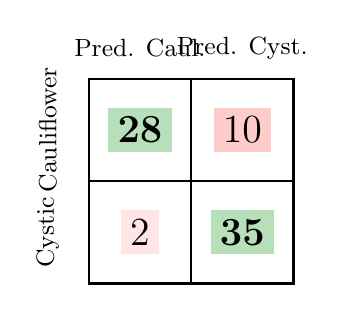
\begin{tikzpicture}[scale=1.3]
                    \draw[thick] (0,0) rectangle (2,2);
                    \draw[thick] (1,0) -- (1,2);
                    \draw[thick] (0,1) -- (2,1);
                    
                    \node[fill=cysticGreen!40] at (0.5,1.5) {\Large\textbf{28}};
                    \node[fill=red!20] at (1.5,1.5) {\Large 10};
                    \node[fill=red!10] at (0.5,0.5) {\Large 2};
                    \node[fill=cysticGreen!40] at (1.5,0.5) {\Large\textbf{35}};
                    
                    \node[rotate=90] at (-0.4,1.5) {\small Cauliflower};
                    \node[rotate=90] at (-0.4,0.5) {\small Cystic};
                    \node at (0.5,2.3) {\small Pred. Caul.};
                    \node at (1.5,2.3) {\small Pred. Cyst.};
                \end{tikzpicture}
            \end{center}
        \end{column}
        \begin{column}{0.5\textwidth}
            \textbf{Results:}
            \begin{itemize}
                \item 63/75 correct = \textbf{84\%}
                \item TP Cauliflower: 28
                \item TP Cystic: 35
            \end{itemize}
            
            \vspace{0.5em}
            \textbf{Main Error Pattern:}\\
            Cauliflower $\rightarrow$ Cystic (10 cases)
            
            \vspace{0.5em}
            \textbf{Interpretation:}
            \begin{itemize}
                \item Low-deformation cauliflowers
                \item Quasi-spherical appearance
                \item Possible transitional phenotypes
            \end{itemize}
        \end{column}
    \end{columns}
\end{frame}

% Slide 35: Transfer Learning Impact
\begin{frame}{Transfer Learning Impact}
    \begin{columns}
        \begin{column}{0.5\textwidth}
    \begin{table}
        \centering
        \begin{tabular}{lc}
            \toprule
                    \textbf{Strategy} & \textbf{Accuracy} \\
            \midrule
                    GAT from scratch & 76\% \\
                    GAT pre-trained & \textbf{84\%} \\
            \midrule
            \textit{Improvement} & \textbf{+8\%} \\
            \bottomrule
        \end{tabular}
    \end{table}
    
            \vspace{0.5em}
    \textbf{Data Efficiency:}
    \begin{itemize}
                \item Pre-trained + 25\% data: 78\%
                \item From-scratch + 100\%: 76\%
    \end{itemize}
    
            $\Rightarrow$ \textbf{4× fewer annotations needed!}
        \end{column}
        \begin{column}{0.5\textwidth}
            \begin{center}
                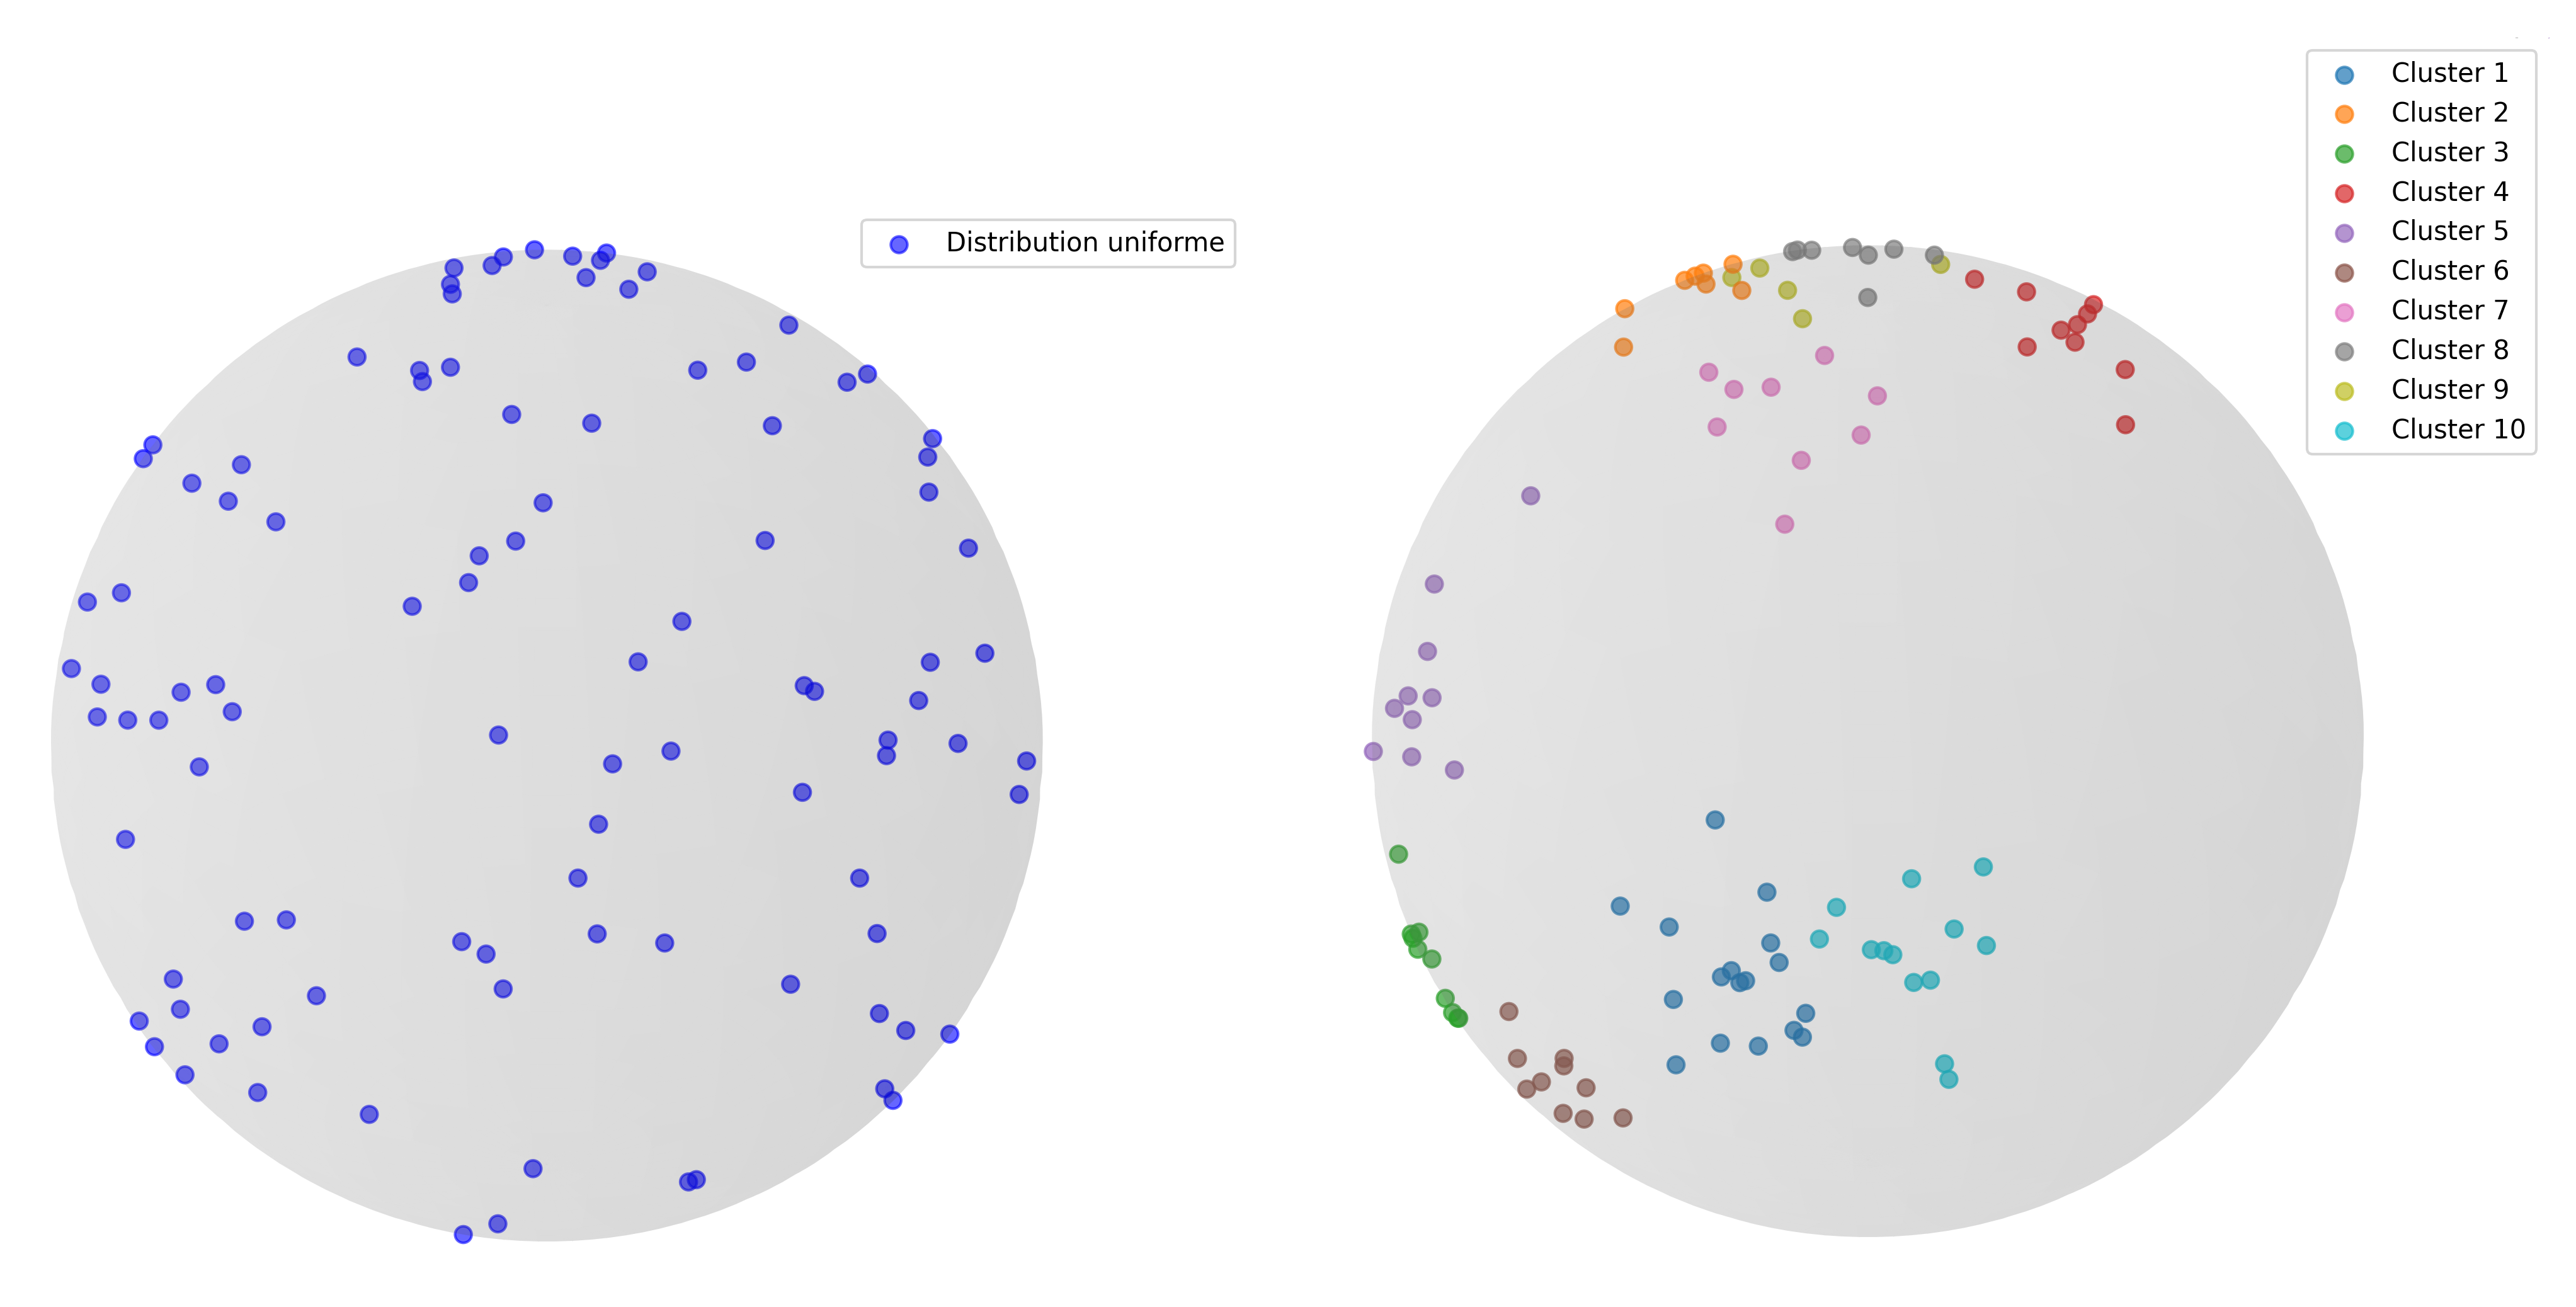
\includegraphics[width=\textwidth]{img/distrib2.png}\\
                {\footnotesize Data efficiency comparison}
            \end{center}
            
            \vspace{0.3em}
            \textbf{Convergence:} 3× faster
        \end{column}
    \end{columns}
\end{frame}

% Slide 36: Final Architecture
\begin{frame}{Final Architecture}
    \begin{center}
        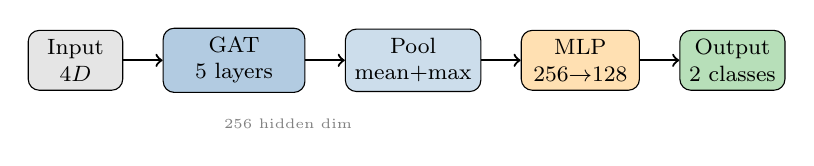
\begin{tikzpicture}[
            node distance=0.5cm,
            block/.style={rectangle, rounded corners, draw, minimum height=0.7cm, align=center, font=\footnotesize},
            arrow/.style={->, thick}
        ]
            \node[block, fill=gray!20, minimum width=1.2cm] (input) {Input\\$4D$};
            \node[block, fill=inriaBlue!30, minimum width=1.8cm, right=of input] (gat) {GAT\\5 layers};
            \node[block, fill=inriaBlue!20, minimum width=1.5cm, right=of gat] (pool) {Pool\\mean+max};
            \node[block, fill=cauliflowerOrange!30, minimum width=1.5cm, right=of pool] (mlp) {MLP\\256$\rightarrow$128};
            \node[block, fill=cysticGreen!40, minimum width=1.2cm, right=of mlp] (out) {Output\\2 classes};
            
            \draw[arrow] (input) -- (gat);
            \draw[arrow] (gat) -- (pool);
            \draw[arrow] (pool) -- (mlp);
            \draw[arrow] (mlp) -- (out);
            
            \node[font=\tiny, text=gray] at (2.7,-0.8) {256 hidden dim};
        \end{tikzpicture}
    \end{center}
    
    \vspace{0.3em}
    \begin{columns}
        \begin{column}{0.5\textwidth}
            \begin{table}
                \footnotesize
                \begin{tabular}{ll}
                    \toprule
                    \multicolumn{2}{c}{\textbf{Training}} \\
                    \midrule
                    Optimizer & AdamW \\
                    LR (pre-train) & $10^{-3}$ \\
                    LR (fine-tune) & $10^{-4}$ \\
                    \bottomrule
                \end{tabular}
            \end{table}
        \end{column}
        \begin{column}{0.5\textwidth}
            \begin{table}
                \footnotesize
                \begin{tabular}{ll}
                    \toprule
                    \multicolumn{2}{c}{\textbf{Inference}} \\
                    \midrule
                    Speed & 200+ org/min \\
                    Memory & $\sim$8 GB GPU \\
                    Hardware & RTX 3080 \\
                    \bottomrule
                \end{tabular}
            \end{table}
        \end{column}
    \end{columns}
\end{frame}

% Slide: Learning Curves Detail
\begin{frame}{Learning Curves: Detailed Analysis}
    \begin{columns}
        \begin{column}{0.5\textwidth}
            \textbf{Data Efficiency Gains:}
            \begin{table}
                \footnotesize
                \begin{tabular}{lcc}
                    \toprule
                    \textbf{Data \%} & \textbf{From-scratch} & \textbf{Pre-trained} \\
                    \midrule
                    10\% & 58\% & 71\% (\textcolor{cysticGreen}{+13\%}) \\
                    25\% & 67\% & 78\% (\textcolor{cysticGreen}{+11\%}) \\
                    50\% & 72\% & 82\% (\textcolor{cysticGreen}{+10\%}) \\
                    100\% & 76\% & 84\% (\textcolor{cysticGreen}{+8\%}) \\
                    \bottomrule
                \end{tabular}
            \end{table}
            
            \vspace{0.5em}
            \textbf{Key Observation:}\\
            Largest gains at \textbf{low data} regime
        \end{column}
        \begin{column}{0.5\textwidth}
            \textbf{Convergence Speed:}
            \begin{itemize}
                \item Pre-trained: \textbf{20-30 epochs}
                \item From-scratch: 80-100 epochs
                \item $\Rightarrow$ \textbf{3× faster}
            \end{itemize}
            
            \vspace{0.5em}
            \textbf{Implication:}\\
            Synthetic pre-training teaches useful representations of spatial organization
            
            \vspace{0.5em}
            \textbf{Practical Impact:}\\
            125 real organoids (pre-trained) $\approx$\\
            500 real organoids (from-scratch)
        \end{column}
    \end{columns}
\end{frame}

% Slide: Computational Efficiency
\begin{frame}{Computational Efficiency}
    \begin{columns}
        \begin{column}{0.5\textwidth}
            \textbf{Inference Performance:}
            \begin{itemize}
                \item \textbf{200+ organoids/minute}
                \item GPU batch processing
                \item Enables high-throughput screening
            \end{itemize}
            
            \vspace{0.5em}
            \textbf{Memory Footprint:}
            \begin{itemize}
                \item $\sim$8 GB GPU memory
                \item Compatible with standard hardware
                \item RTX 3080 / A100
            \end{itemize}
        \end{column}
        \begin{column}{0.5\textwidth}
            \textbf{Reproducibility:}
            \begin{itemize}
                \item \textbf{100\% deterministic}
                \item No inter-observer variability
                \item Identical results every run
            \end{itemize}
            
            \vspace{0.5em}
            \textbf{Scalability:}
            \begin{table}
                \footnotesize
                \begin{tabular}{lc}
                    \toprule
                    \textbf{Organoids} & \textbf{Time} \\
                    \midrule
                    100 & $\sim$30 sec \\
                    1,000 & $\sim$5 min \\
                    10,000 & $\sim$50 min \\
                    \bottomrule
                \end{tabular}
            \end{table}
        \end{column}
    \end{columns}
    
    \vspace{0.3em}
    \begin{block}{vs Manual Analysis}
        \textbf{Manual:} 30 min/organoid $\times$ 1000 = 500 hours\\
        \textbf{Automated:} 5 min total — \textbf{6000× faster}
    \end{block}
\end{frame}

% Slide 37: Limitations
\begin{frame}{Identified Limitations}
    \begin{itemize}
        \item \textbf{Segmentation dependency:} Errors propagate through pipeline
        
        \vspace{0.5em}
        \item \textbf{Validation scope:} Prostate organoids only; generalization needs testing
        
        \vspace{0.5em}
        \item \textbf{No inter-laboratory validation:} Different microscopes, protocols
        
        \vspace{0.5em}
        \item \textbf{No interpretability analysis:} Which cells drive predictions?
        \end{itemize}
\end{frame}

% Slide 38: Part IV Summary
\begin{frame}{Part IV Summary: Results}
    \begin{enumerate}
        \item \textbf{GAT achieves best performance:}
    \begin{itemize}
            \item 84\% accuracy on real data
            \item MSE 0.118 on synthetic data
        \end{itemize}
        
        \vspace{0.5em}
        \item \textbf{Transfer learning is transformative:}
        \begin{itemize}
            \item +8\% accuracy improvement
            \item 4× data efficiency
            \item 3× faster convergence
        \end{itemize}
        
        \vspace{0.5em}
        \item \textbf{Practical system:}
        \begin{itemize}
            \item 200+ organoids/minute inference
            \item Fully automated, reproducible
        \end{itemize}
    \end{enumerate}
\end{frame}

% =============================================================================
% CONCLUSION
% =============================================================================
\section{Conclusion}

\begin{frame}
    \begin{center}
        {\Huge \textbf{Conclusion}}\\[1em]
        {\LARGE Contributions \& Perspectives}
    \end{center}
\end{frame}

% Slide: Contribution 1
\begin{frame}{Contribution 1: Graph-Based Representation}
    \begin{block}{Geometric Graphs for Organoid Modeling}
        From raw 3D images to compact graph representations
    \end{block}
    
    \vspace{0.5em}
    \begin{columns}
        \begin{column}{0.5\textwidth}
            \textbf{Key Innovation:}
            \begin{itemize}
                \item Cell $\rightarrow$ Node abstraction
                \item Spatial proximity $\rightarrow$ Edges
                \item 4D features (position + volume)
            \end{itemize}
            
            \vspace{0.5em}
            \textbf{Impact:}
            \begin{itemize}
                \item \textbf{1000× compression}
                \item Preserves biological structure
                \item Enables GNN analysis
            \end{itemize}
        \end{column}
        \begin{column}{0.5\textwidth}
            \begin{center}
                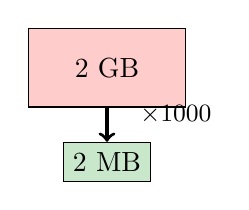
\begin{tikzpicture}[scale=0.6]
                    \node[rectangle, draw, fill=red!20, minimum width=2cm, minimum height=1cm] (img) at (0,2) {2 GB};
                    \node[rectangle, draw, fill=cysticGreen!30, minimum width=1cm, minimum height=0.5cm] (graph) at (0,0) {2 MB};
                    \draw[->, very thick] (img) -- (graph);
                    \node[right] at (0.5,1) {\small $\times 1000$};
                \end{tikzpicture}
            \end{center}
        \end{column}
    \end{columns}
\end{frame}

% Slide: Contribution 2
\begin{frame}{Contribution 2: GRETSI Comparative Study}
    \begin{block}{Published at GRETSI 2025}
        Rigorous comparison: GNNs vs Spatial Statistics
    \end{block}
    
    \vspace{0.5em}
    \begin{columns}
        \begin{column}{0.5\textwidth}
            \textbf{Key Findings:}
            \begin{itemize}
                \item GNNs: better \textbf{geometric generalization}
                \item Spatial stats: better \textbf{noise robustness}
            \end{itemize}
            
            \vspace{0.5em}
            \textbf{Recommendation:}\\
            GNNs for variable morphologies\\
            Statistics for idealized conditions
        \end{column}
        \begin{column}{0.5\textwidth}
            \textbf{Impact:}
            \begin{itemize}
                \item Guides method selection
                \item Justifies deep learning approach
                \item Foundation for thesis methodology
            \end{itemize}
            
            \vspace{0.5em}
            \textbf{Citation:}\\
            {\footnotesize Martin et al., GRETSI 2025}
        \end{column}
    \end{columns}
\end{frame}

% Slide: Contribution 3
\begin{frame}{Contribution 3: Synthetic Data Generation}
    \begin{block}{Point Process-Based Generation}
        Poisson + Matérn processes for synthetic organoids
    \end{block}
    
    \vspace{0.5em}
    \begin{columns}
        \begin{column}{0.5\textwidth}
            \textbf{Method:}
            \begin{itemize}
                \item Poisson $\rightarrow$ Cystic (uniform)
                \item Matérn $\rightarrow$ Cauliflower (clustered)
            \end{itemize}
            
            \vspace{0.5em}
            \textbf{Scale:}
            \begin{itemize}
                \item \textbf{100,000} synthetic organoids
                \item Perfect ground truth labels
                \item Controllable difficulty
            \end{itemize}
        \end{column}
        \begin{column}{0.5\textwidth}
            \textbf{Impact:}
            \begin{itemize}
                \item Enabled research without real data
                \item Foundation for transfer learning
                \item +8\% accuracy improvement
            \end{itemize}
            
            \vspace{0.5em}
            \textbf{Generalizable:}\\
            Applicable to other spherical/ellipsoidal biological structures
        \end{column}
    \end{columns}
\end{frame}

% Slide: Contribution 4
\begin{frame}{Contribution 4: Transfer Learning Strategy}
    \begin{block}{Synthetic $\rightarrow$ Real Transfer}
        Pre-train on synthetic, fine-tune on real
    \end{block}
    
    \vspace{0.5em}
    \textbf{Results:}
    \begin{columns}
        \begin{column}{0.33\textwidth}
            \begin{center}
                {\Large \textbf{+8\%}}\\
                Accuracy improvement
            \end{center}
        \end{column}
        \begin{column}{0.33\textwidth}
            \begin{center}
                {\Large \textbf{4×}}\\
                Data efficiency
            \end{center}
        \end{column}
        \begin{column}{0.33\textwidth}
            \begin{center}
                {\Large \textbf{3×}}\\
                Faster convergence
            \end{center}
        \end{column}
    \end{columns}
    
    \vspace{0.5em}
    \begin{alertblock}{Practical Impact}
        125 organoids (pre-trained) = 500 organoids (from-scratch)\\
        \textbf{Transforms annotation requirements}
    \end{alertblock}
\end{frame}

% Slide: Contribution 5
\begin{frame}{Contribution 5: Complete Automated Pipeline}
    \begin{block}{End-to-End System}
        From raw 3D images to phenotype predictions
    \end{block}
    
    \vspace{0.5em}
    \begin{columns}
        \begin{column}{0.5\textwidth}
            \textbf{Components:}
            \begin{itemize}
                \item Preprocessing
                \item Faster Cellpose (5× speedup)
                \item Graph construction
                \item GNN classification
            \end{itemize}
        \end{column}
        \begin{column}{0.5\textwidth}
            \textbf{Properties:}
            \begin{itemize}
                \item \textbf{Fully automated}
                \item \textbf{200+ organoids/minute}
                \item \textbf{Open-source}
                \item Reproducible
            \end{itemize}
        \end{column}
    \end{columns}
    
    \vspace{0.5em}
    \begin{center}
        \textbf{Code available:} \url{github.com/morpheme-inria/organoid-gnn}
    \end{center}
\end{frame}

% Slide: Short-term Perspectives
\begin{frame}{Short-Term Perspectives}
    \begin{columns}
        \begin{column}{0.5\textwidth}
            \textbf{Methodological Extensions:}
            \begin{itemize}
                \item Multi-scale graphs\\{\footnotesize (cell → region → organoid)}
                \item Graph Transformers\\{\footnotesize (global attention mechanism)}
                \item Interpretability analysis\\{\footnotesize (which cells drive predictions?)}
            \end{itemize}
        \end{column}
        \begin{column}{0.5\textwidth}
            \textbf{Multi-Modal Integration:}
            \begin{itemize}
                \item Spatial transcriptomics + imaging
                \item Temporal data from time-lapse
                \item Metabolomic features
            \end{itemize}
            
            \vspace{0.5em}
            \textbf{Clinical Validation:}
            \begin{itemize}
                \item Prospective patient cohorts
                \item Multi-site testing
            \end{itemize}
        \end{column}
    \end{columns}
\end{frame}

% Slide: Long-term Perspectives
\begin{frame}{Long-Term Vision}
    \begin{columns}
        \begin{column}{0.5\textwidth}
            \textbf{Therapeutic Response Prediction:}
            \begin{itemize}
                \item Patient-derived organoids
                \item Test treatments in silico
                \item Personalized therapy selection
            \end{itemize}
            
            \vspace{0.5em}
            \textbf{Generative Graph Models:}
            \begin{itemize}
                \item In silico organoid design
                \item Optimize culture protocols
                \item Computational biology
            \end{itemize}
        \end{column}
        \begin{column}{0.5\textwidth}
            \textbf{Multi-Organ Extension:}
            \begin{itemize}
                \item Brain organoids
                \item Liver, kidney, lung
                \item Tumor organoids
            \end{itemize}
            
            \vspace{0.5em}
            \textbf{Societal Impact:}
            \begin{itemize}
                \item \textbf{3Rs principles}\\{\footnotesize Replace, Reduce, Refine}
                \item Accelerate drug discovery
                \item Reduce animal testing
            \end{itemize}
        \end{column}
    \end{columns}
\end{frame}

% Slide 42: Final Message
\begin{frame}{Final Message}
    \begin{center}
        \textbf{\Large Geometric Graph Neural Networks}\\
        are a powerful tool for 3D organoid analysis
        
        \vspace{1em}
        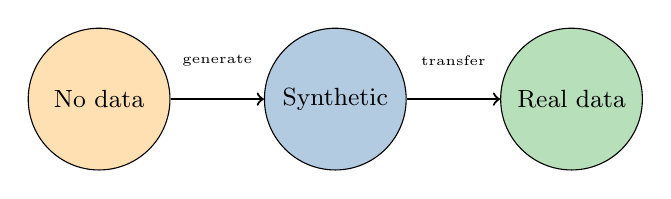
\begin{tikzpicture}
            \node[draw, circle, fill=cauliflowerOrange!30, minimum size=1.8cm] (no) at (0,0) {\small No data};
            \node[draw, circle, fill=inriaBlue!30, minimum size=1.8cm] (synth) at (3,0) {\small Synthetic};
            \node[draw, circle, fill=cysticGreen!40, minimum size=1.8cm] (real) at (6,0) {\small Real data};
            \draw[->, thick] (no) -- (synth);
            \draw[->, thick] (synth) -- (real);
            \node[above] at (1.5,0.3) {\tiny generate};
            \node[above] at (4.5,0.3) {\tiny transfer};
        \end{tikzpicture}
        
        \vspace{1em}
        \textbf{Open-source code} available for the community
        
        \vspace{1em}
        {\Large Thank you for your attention.}\\
        {\large I am happy to take your questions.}
    \end{center}
\end{frame}

% =============================================================================
% BACKUP SLIDES
% =============================================================================
\appendix

\begin{frame}
    \begin{center}
        {\Huge Backup Slides}
    \end{center}
\end{frame}

\begin{frame}{Confusion Matrix (Detail)}
    \begin{center}
        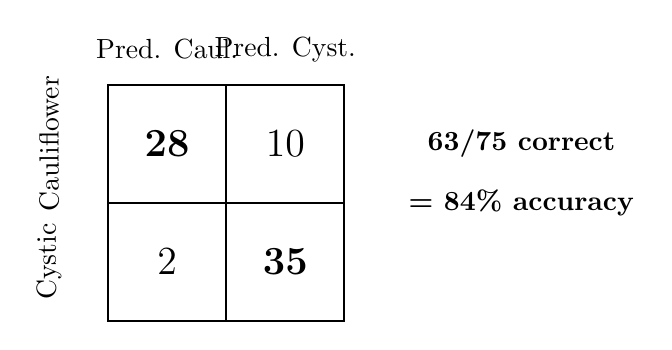
\begin{tikzpicture}[scale=1.5]
            \draw[thick] (0,0) rectangle (2,2);
            \draw[thick] (1,0) -- (1,2);
            \draw[thick] (0,1) -- (2,1);
            
            \node at (0.5,1.5) {\Large\textbf{28}};
            \node at (1.5,1.5) {\Large 10};
            \node at (0.5,0.5) {\Large 2};
            \node at (1.5,0.5) {\Large\textbf{35}};
            
            \node[rotate=90] at (-0.5,1.5) {Cauliflower};
            \node[rotate=90] at (-0.5,0.5) {Cystic};
            \node at (0.5,2.3) {Pred. Caul.};
            \node at (1.5,2.3) {Pred. Cyst.};
            
            \node at (3.5,1.5) {\textbf{63/75 correct}};
            \node at (3.5,1) {\textbf{= 84\% accuracy}};
        \end{tikzpicture}
    \end{center}
\end{frame}

\begin{frame}{Anticipated Questions}
    \begin{enumerate}
        \item \textbf{Why GAT over EGNN?}\\
        Trade-off: GAT wins on accuracy; EGNN wins on guarantees
        
        \vspace{0.5em}
        \item \textbf{Synthetic data validation?}\\
        Empirical gains (+8\%) demonstrate practical utility
        
        \vspace{0.5em}
        \item \textbf{Generalization to other organoids?}\\
        Principles transferable; requires fine-tuning Cellpose
        
        \vspace{0.5em}
        \item \textbf{Why only 500 organoids?}\\
        Quality over quantity — ensuring label-morphology consistency
        
        \vspace{0.5em}
        \item \textbf{Clinical deployment?}\\
        Would require regulatory validation (IVDR/FDA)
    \end{enumerate}
\end{frame}

\begin{frame}{EGNN Formulas (Detail)}
    \textbf{Message computation} (invariant):
    \begin{equation*}
        m_{ij} = \phi_m\left(h_i, h_j, \|x_i - x_j\|^2\right)
    \end{equation*}
    
    \textbf{Coordinate update} (equivariant):
    \begin{equation*}
        x_i^{(l+1)} = x_i^{(l)} + \sum_{j \neq i} (x_i - x_j) \cdot \phi_x(m_{ij})
    \end{equation*}
    
    \textbf{Feature update}:
    \begin{equation*}
        h_i^{(l+1)} = \phi_h\left(h_i^{(l)}, \sum_{j \in \mathcal{N}(i)} m_{ij}\right)
    \end{equation*}
    
    \begin{block}{Property}
        Invariant messages + Equivariant coordinate updates = E(3)-equivariant network
    \end{block}
\end{frame}

\begin{frame}{Timing Checkpoints}
    \begin{table}
        \centering
        \begin{tabular}{lc}
            \toprule
            \textbf{Section} & \textbf{Target Time} \\
            \midrule
            After Introduction (Slide 6) & $\sim$5 min \\
            After Part I - Justification (Slide 14) & $\sim$15 min \\
            After Part II - GNN Theory (Slide 24) & $\sim$25 min \\
            After Part III - Pipeline (Slide 30) & $\sim$32 min \\
            After Part IV - Results (Slide 38) & $\sim$42 min \\
            End & $\sim$45 min \\
            \bottomrule
        \end{tabular}
    \end{table}
    
    \vspace{1em}
    \textbf{If running long:} Abbreviate EGNN details\\
    \textbf{If running short:} Expand perspectives and limitations
\end{frame}

\end{document}
